\documentclass[1p]{elsarticle_modified}
%\bibliographystyle{elsarticle-num}

%\usepackage[colorlinks]{hyperref}
%\usepackage{abbrmath_seonhwa} %\Abb, \Ascr, \Acal ,\Abf, \Afrak
\usepackage{amsfonts}
\usepackage{amssymb}
\usepackage{amsmath}
\usepackage{amsthm}
\usepackage{scalefnt}
\usepackage{amsbsy}
\usepackage{kotex}
\usepackage{caption}
\usepackage{subfig}
\usepackage{color}
\usepackage{graphicx}
\usepackage{xcolor} %% white, black, red, green, blue, cyan, magenta, yellow
\usepackage{float}
\usepackage{setspace}
\usepackage{hyperref}

\usepackage{tikz}
\usetikzlibrary{arrows}

\usepackage{multirow}
\usepackage{array} % fixed length table
\usepackage{hhline}

%%%%%%%%%%%%%%%%%%%%%
\makeatletter
\renewcommand*\env@matrix[1][\arraystretch]{%
	\edef\arraystretch{#1}%
	\hskip -\arraycolsep
	\let\@ifnextchar\new@ifnextchar
	\array{*\c@MaxMatrixCols c}}
\makeatother %https://tex.stackexchange.com/questions/14071/how-can-i-increase-the-line-spacing-in-a-matrix
%%%%%%%%%%%%%%%

\usepackage[normalem]{ulem}

\newcommand{\msout}[1]{\ifmmode\text{\sout{\ensuremath{#1}}}\else\sout{#1}\fi}
%SOURCE: \msout is \stkout macro in https://tex.stackexchange.com/questions/20609/strikeout-in-math-mode

\newcommand{\cancel}[1]{
	\ifmmode
	{\color{red}\msout{#1}}
	\else
	{\color{red}\sout{#1}}
	\fi
}

\newcommand{\add}[1]{
	{\color{blue}\uwave{#1}}
}

\newcommand{\replace}[2]{
	\ifmmode
	{\color{red}\msout{#1}}{\color{blue}\uwave{#2}}
	\else
	{\color{red}\sout{#1}}{\color{blue}\uwave{#2}}
	\fi
}

\newcommand{\Sol}{\mathcal{S}} %segment
\newcommand{\D}{D} %diagram
\newcommand{\A}{\mathcal{A}} %arc


%%%%%%%%%%%%%%%%%%%%%%%%%%%%%5 test

\def\sl{\operatorname{\textup{SL}}(2,\Cbb)}
\def\psl{\operatorname{\textup{PSL}}(2,\Cbb)}
\def\quan{\mkern 1mu \triangleright \mkern 1mu}

\theoremstyle{definition}
\newtheorem{thm}{Theorem}[section]
\newtheorem{prop}[thm]{Proposition}
\newtheorem{lem}[thm]{Lemma}
\newtheorem{ques}[thm]{Question}
\newtheorem{cor}[thm]{Corollary}
\newtheorem{defn}[thm]{Definition}
\newtheorem{exam}[thm]{Example}
\newtheorem{rmk}[thm]{Remark}
\newtheorem{alg}[thm]{Algorithm}

\newcommand{\I}{\sqrt{-1}}
\begin{document}

%\begin{frontmatter}
%
%\title{Boundary parabolic representations of knots up to 8 crossings}
%
%%% Group authors per affiliation:
%\author{Yunhi Cho} 
%\address{Department of Mathematics, University of Seoul, Seoul, Korea}
%\ead{yhcho@uos.ac.kr}
%
%
%\author{Seonhwa Kim} %\fnref{s_kim}}
%\address{Center for Geometry and Physics, Institute for Basic Science, Pohang, 37673, Korea}
%\ead{ryeona17@ibs.re.kr}
%
%\author{Hyuk Kim}
%\address{Department of Mathematical Sciences, Seoul National University, Seoul 08826, Korea}
%\ead{hyukkim@snu.ac.kr}
%
%\author{Seokbeom Yoon}
%\address{Department of Mathematical Sciences, Seoul National University, Seoul, 08826,  Korea}
%\ead{sbyoon15@snu.ac.kr}
%
%\begin{abstract}
%We find all boundary parabolic representation of knots up to 8 crossings.
%
%\end{abstract}
%\begin{keyword}
%    \MSC[2010] 57M25 
%\end{keyword}
%
%\end{frontmatter}

%\linenumbers
%\tableofcontents
%
\newcommand\colored[1]{\textcolor{white}{\rule[-0.35ex]{0.8em}{1.4ex}}\kern-0.8em\color{red} #1}%
%\newcommand\colored[1]{\textcolor{white}{ #1}\kern-2.17ex	\textcolor{white}{ #1}\kern-1.81ex	\textcolor{white}{ #1}\kern-2.15ex\color{red}#1	}

{\Large $\underline{12a_{0467}~(K12a_{0467})}$}

\setlength{\tabcolsep}{10pt}
\renewcommand{\arraystretch}{1.6}
\vspace{1cm}\begin{tabular}{m{100pt}>{\centering\arraybackslash}m{274pt}}
\multirow{5}{120pt}{
	\centering
	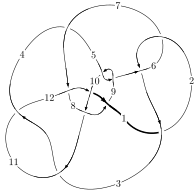
\includegraphics[width=112pt]{../../../GIT/diagram.site/Diagrams/png/1268_12a_0467.png}\\
\ \ \ A knot diagram\footnotemark}&
\allowdisplaybreaks
\textbf{Linearized knot diagam} \\
\cline{2-2}
 &
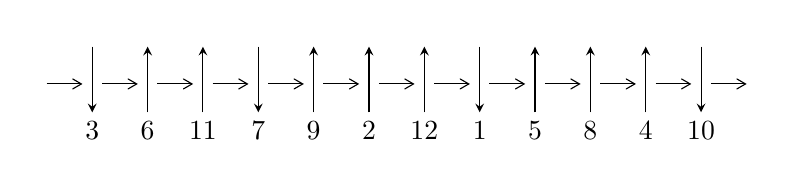
\begin{tikzpicture}[x=20pt, y=17pt]
	% nodes
	\node (C0) at (0, 0) {};
	\node (C1) at (1, 0) {};
	\node (C1U) at (1, +1) {};
	\node (C1D) at (1, -1) {3};

	\node (C2) at (2, 0) {};
	\node (C2U) at (2, +1) {};
	\node (C2D) at (2, -1) {6};

	\node (C3) at (3, 0) {};
	\node (C3U) at (3, +1) {};
	\node (C3D) at (3, -1) {11};

	\node (C4) at (4, 0) {};
	\node (C4U) at (4, +1) {};
	\node (C4D) at (4, -1) {7};

	\node (C5) at (5, 0) {};
	\node (C5U) at (5, +1) {};
	\node (C5D) at (5, -1) {9};

	\node (C6) at (6, 0) {};
	\node (C6U) at (6, +1) {};
	\node (C6D) at (6, -1) {2};

	\node (C7) at (7, 0) {};
	\node (C7U) at (7, +1) {};
	\node (C7D) at (7, -1) {12};

	\node (C8) at (8, 0) {};
	\node (C8U) at (8, +1) {};
	\node (C8D) at (8, -1) {1};

	\node (C9) at (9, 0) {};
	\node (C9U) at (9, +1) {};
	\node (C9D) at (9, -1) {5};

	\node (C10) at (10, 0) {};
	\node (C10U) at (10, +1) {};
	\node (C10D) at (10, -1) {8};

	\node (C11) at (11, 0) {};
	\node (C11U) at (11, +1) {};
	\node (C11D) at (11, -1) {4};

	\node (C12) at (12, 0) {};
	\node (C12U) at (12, +1) {};
	\node (C12D) at (12, -1) {10};
	\node (C13) at (13, 0) {};

	% arrows
	\draw[->,>={angle 60}]
	(C0) edge (C1) (C1) edge (C2) (C2) edge (C3) (C3) edge (C4) (C4) edge (C5) (C5) edge (C6) (C6) edge (C7) (C7) edge (C8) (C8) edge (C9) (C9) edge (C10) (C10) edge (C11) (C11) edge (C12) (C12) edge (C13) ;	\draw[->,>=stealth]
	(C1U) edge (C1D) (C2D) edge (C2U) (C3D) edge (C3U) (C4U) edge (C4D) (C5D) edge (C5U) (C6D) edge (C6U) (C7D) edge (C7U) (C8U) edge (C8D) (C9D) edge (C9U) (C10D) edge (C10U) (C11D) edge (C11U) (C12U) edge (C12D) ;
	\end{tikzpicture} \\
\hhline{~~} \\& 
\textbf{Solving Sequence} \\ \cline{2-2} 
 &
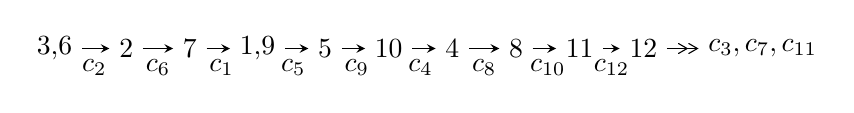
\begin{tikzpicture}[x=23pt, y=7pt]
	% node
	\node (A0) at (-1/8, 0) {3,6};
	\node (A1) at (1, 0) {2};
	\node (A2) at (2, 0) {7};
	\node (A3) at (49/16, 0) {1,9};
	\node (A4) at (33/8, 0) {5};
	\node (A5) at (41/8, 0) {10};
	\node (A6) at (49/8, 0) {4};
	\node (A7) at (57/8, 0) {8};
	\node (A8) at (65/8, 0) {11};
	\node (A9) at (73/8, 0) {12};
	\node (C1) at (1/2, -1) {$c_{2}$};
	\node (C2) at (3/2, -1) {$c_{6}$};
	\node (C3) at (5/2, -1) {$c_{1}$};
	\node (C4) at (29/8, -1) {$c_{5}$};
	\node (C5) at (37/8, -1) {$c_{9}$};
	\node (C6) at (45/8, -1) {$c_{4}$};
	\node (C7) at (53/8, -1) {$c_{8}$};
	\node (C8) at (61/8, -1) {$c_{10}$};
	\node (C9) at (69/8, -1) {$c_{12}$};
	\node (A10) at (11, 0) {$c_{3},c_{7},c_{11}$};

	% edge
	\draw[->,>=stealth]	
	(A0) edge (A1) (A1) edge (A2) (A2) edge (A3) (A3) edge (A4) (A4) edge (A5) (A5) edge (A6) (A6) edge (A7) (A7) edge (A8) (A8) edge (A9) ;
	\draw[->>,>={angle 60}]	
	(A9) edge (A10);
\end{tikzpicture} \\ 

\end{tabular} \\

\footnotetext{
The image of knot diagram is generated by the software ``\textbf{Draw programme}" developed by Andrew Bartholomew(\url{http://www.layer8.co.uk/maths/draw/index.htm\#Running-draw}), where we modified some parts for our purpose(\url{https://github.com/CATsTAILs/LinksPainter}).
}\phantom \\ \newline 
\centering \textbf{Ideals for irreducible components\footnotemark of $X_{\text{par}}$} 
 
\begin{align*}
I^u_{1}&=\langle 
2.43654\times10^{731} u^{186}+4.54915\times10^{731} u^{185}+\cdots+3.47272\times10^{730} b-6.08362\times10^{734},\\
\phantom{I^u_{1}}&\phantom{= \langle  }1.83544\times10^{733} u^{186}+6.31204\times10^{733} u^{185}+\cdots+1.39951\times10^{733} a+1.20246\times10^{737},\\
\phantom{I^u_{1}}&\phantom{= \langle  }u^{187}+3 u^{186}+\cdots+10920 u+5239\rangle \\
I^u_{2}&=\langle 
-2.84748\times10^{20} u^{51}+3.83075\times10^{20} u^{50}+\cdots+1.55518\times10^{19} b-6.54423\times10^{19},\\
\phantom{I^u_{2}}&\phantom{= \langle  }-2.20974\times10^{18} u^{51}+1.43753\times10^{19} u^{50}+\cdots+8.18517\times10^{17} a+2.27369\times10^{19},\;u^{52}-2 u^{51}+\cdots+2 u+1\rangle \\
\\
\end{align*}
\raggedright * 2 irreducible components of $\dim_{\mathbb{C}}=0$, with total 239 representations.\\
\footnotetext{All coefficients of polynomials are rational numbers. But the coefficients are sometimes approximated in decimal forms when there is not enough margin.}
\newpage
\renewcommand{\arraystretch}{1}
\centering \section*{I. $I^u_{1}= \langle 2.44\times10^{731} u^{186}+4.55\times10^{731} u^{185}+\cdots+3.47\times10^{730} b-6.08\times10^{734},\;1.84\times10^{733} u^{186}+6.31\times10^{733} u^{185}+\cdots+1.40\times10^{733} a+1.20\times10^{737},\;u^{187}+3 u^{186}+\cdots+10920 u+5239 \rangle$}
\flushleft \textbf{(i) Arc colorings}\\
\begin{tabular}{m{7pt} m{180pt} m{7pt} m{180pt} }
\flushright $a_{3}=$&$\begin{pmatrix}1\\0\end{pmatrix}$ \\
\flushright $a_{6}=$&$\begin{pmatrix}0\\u\end{pmatrix}$ \\
\flushright $a_{2}=$&$\begin{pmatrix}1\\u^2\end{pmatrix}$ \\
\flushright $a_{7}=$&$\begin{pmatrix}u\\u^3+u\end{pmatrix}$ \\
\flushright $a_{1}=$&$\begin{pmatrix}u^2+1\\u^2\end{pmatrix}$ \\
\flushright $a_{9}=$&$\begin{pmatrix}-1.31149 u^{186}-4.51019 u^{185}+\cdots-19216.4 u-8592.00\\-7.01622 u^{186}-13.0997 u^{185}+\cdots-17093.4 u+17518.3\end{pmatrix}$ \\
\flushright $a_{5}=$&$\begin{pmatrix}-4.05296 u^{186}-8.70148 u^{185}+\cdots-20947.1 u+2815.98\\4.55158 u^{186}+18.8011 u^{185}+\cdots+87737.8 u+46534.4\end{pmatrix}$ \\
\flushright $a_{10}=$&$\begin{pmatrix}3.28956 u^{186}+13.0121 u^{185}+\cdots+60174.6 u+31327.3\\2.37109 u^{186}+6.69340 u^{185}+\cdots+24665.2 u+8314.07\end{pmatrix}$ \\
\flushright $a_{4}=$&$\begin{pmatrix}-14.7745 u^{186}-38.3820 u^{185}+\cdots-120348. u-25763.8\\1.85301 u^{186}+5.37884 u^{185}+\cdots+17379.0 u+4939.63\end{pmatrix}$ \\
\flushright $a_{8}=$&$\begin{pmatrix}-2.56385 u^{186}-12.6576 u^{185}+\cdots-66579.2 u-39277.1\\-0.572985 u^{186}+1.16346 u^{185}+\cdots+15839.8 u+13975.7\end{pmatrix}$ \\
\flushright $a_{11}=$&$\begin{pmatrix}24.0575 u^{186}+89.6144 u^{185}+\cdots+385976. u+191331.\\-2.77086 u^{186}-2.77145 u^{185}+\cdots+10609.9 u+20101.8\end{pmatrix}$ \\
\flushright $a_{12}=$&$\begin{pmatrix}-9.95948 u^{186}-35.4824 u^{185}+\cdots-148583. u-72494.9\\-3.26650 u^{186}-9.27568 u^{185}+\cdots-30007.3 u-9369.12\end{pmatrix}$\\&\end{tabular}
\flushleft \textbf{(ii) Obstruction class $= -1$}\\~\\
\flushleft \textbf{(iii) Cusp Shapes $= 37.8564 u^{186}+98.0987 u^{185}+\cdots+289617. u+60810.4$}\\~\\
\newpage\renewcommand{\arraystretch}{1}
\flushleft \textbf{(iv) u-Polynomials at the component}\newline \\
\begin{tabular}{m{50pt}|m{274pt}}
Crossings & \hspace{64pt}u-Polynomials at each crossing \\
\hline $$\begin{aligned}c_{1}\end{aligned}$$&$\begin{aligned}
&u^{187}+91 u^{186}+\cdots-674755484 u-27447121
\end{aligned}$\\
\hline $$\begin{aligned}c_{2},c_{6}\end{aligned}$$&$\begin{aligned}
&u^{187}-3 u^{186}+\cdots+10920 u-5239
\end{aligned}$\\
\hline $$\begin{aligned}c_{3},c_{11}\end{aligned}$$&$\begin{aligned}
&u^{187}+u^{186}+\cdots+88574 u-18569
\end{aligned}$\\
\hline $$\begin{aligned}c_{4}\end{aligned}$$&$\begin{aligned}
&u^{187}-9 u^{186}+\cdots+103686897391 u-29441432969
\end{aligned}$\\
\hline $$\begin{aligned}c_{5},c_{9}\end{aligned}$$&$\begin{aligned}
&u^{187}+54 u^{185}+\cdots-82696 u-12769
\end{aligned}$\\
\hline $$\begin{aligned}c_{7}\end{aligned}$$&$\begin{aligned}
&u^{187}-3 u^{186}+\cdots+26048247 u-2479855
\end{aligned}$\\
\hline $$\begin{aligned}c_{8}\end{aligned}$$&$\begin{aligned}
&u^{187}+3 u^{186}+\cdots-1136700959 u-173953039
\end{aligned}$\\
\hline $$\begin{aligned}c_{10}\end{aligned}$$&$\begin{aligned}
&u^{187}+13 u^{186}+\cdots+29 u+1
\end{aligned}$\\
\hline $$\begin{aligned}c_{12}\end{aligned}$$&$\begin{aligned}
&u^{187}-15 u^{186}+\cdots+1290 u-59
\end{aligned}$\\
\hline
\end{tabular}\\~\\
\newpage\renewcommand{\arraystretch}{1}
\flushleft \textbf{(v) Riley Polynomials at the component}\newline \\
\begin{tabular}{m{50pt}|m{274pt}}
Crossings & \hspace{64pt}Riley Polynomials at each crossing \\
\hline $$\begin{aligned}c_{1}\end{aligned}$$&$\begin{aligned}
&y^{187}+31 y^{186}+\cdots-59316051338052392 y-753344451188641
\end{aligned}$\\
\hline $$\begin{aligned}c_{2},c_{6}\end{aligned}$$&$\begin{aligned}
&y^{187}+91 y^{186}+\cdots-674755484 y-27447121
\end{aligned}$\\
\hline $$\begin{aligned}c_{3},c_{11}\end{aligned}$$&$\begin{aligned}
&y^{187}-115 y^{186}+\cdots+15824267086 y-344807761
\end{aligned}$\\
\hline $$\begin{aligned}c_{4}\end{aligned}$$&$\begin{aligned}
&y^{187}+33 y^{186}+\cdots-1.86\times10^{22} y-8.67\times10^{20}
\end{aligned}$\\
\hline $$\begin{aligned}c_{5},c_{9}\end{aligned}$$&$\begin{aligned}
&y^{187}+108 y^{186}+\cdots-13757691970 y-163047361
\end{aligned}$\\
\hline $$\begin{aligned}c_{7}\end{aligned}$$&$\begin{aligned}
&y^{187}-27 y^{186}+\cdots+413324628737959 y-6149680821025
\end{aligned}$\\
\hline $$\begin{aligned}c_{8}\end{aligned}$$&$\begin{aligned}
&y^{187}-19 y^{186}+\cdots+1604876724149993791 y-30259659777335521
\end{aligned}$\\
\hline $$\begin{aligned}c_{10}\end{aligned}$$&$\begin{aligned}
&y^{187}-27 y^{186}+\cdots-175 y-1
\end{aligned}$\\
\hline $$\begin{aligned}c_{12}\end{aligned}$$&$\begin{aligned}
&y^{187}-19 y^{186}+\cdots-127730 y-3481
\end{aligned}$\\
\hline
\end{tabular}\\~\\
\newpage\flushleft \textbf{(vi) Complex Volumes and Cusp Shapes}
$$\begin{array}{c|c|c}  
\text{Solutions to }I^u_{1}& \I (\text{vol} + \sqrt{-1}CS) & \text{Cusp shape}\\
 \hline 
\begin{aligned}
u &= -0.861550 + 0.516101 I \\
a &= \phantom{-}0.142067 + 0.907004 I \\
b &= \phantom{-}0.514385 - 0.385927 I\end{aligned}
 & \phantom{-}6.05061 - 5.19198 I & \phantom{-0.000000 } 0 \\ \hline\begin{aligned}
u &= -0.861550 - 0.516101 I \\
a &= \phantom{-}0.142067 - 0.907004 I \\
b &= \phantom{-}0.514385 + 0.385927 I\end{aligned}
 & \phantom{-}6.05061 + 5.19198 I & \phantom{-0.000000 } 0 \\ \hline\begin{aligned}
u &= -0.263377 + 0.950076 I \\
a &= -0.035684 - 1.105640 I \\
b &= -1.225960 + 0.421383 I\end{aligned}
 & -1.97781 + 1.65161 I & \phantom{-0.000000 } 0 \\ \hline\begin{aligned}
u &= -0.263377 - 0.950076 I \\
a &= -0.035684 + 1.105640 I \\
b &= -1.225960 - 0.421383 I\end{aligned}
 & -1.97781 - 1.65161 I & \phantom{-0.000000 } 0 \\ \hline\begin{aligned}
u &= \phantom{-}0.654179 + 0.776722 I \\
a &= -1.052210 + 0.586150 I \\
b &= -1.57632 - 0.49206 I\end{aligned}
 & \phantom{-}6.92550 + 3.10741 I & \phantom{-0.000000 } 0 \\ \hline\begin{aligned}
u &= \phantom{-}0.654179 - 0.776722 I \\
a &= -1.052210 - 0.586150 I \\
b &= -1.57632 + 0.49206 I\end{aligned}
 & \phantom{-}6.92550 - 3.10741 I & \phantom{-0.000000 } 0 \\ \hline\begin{aligned}
u &= \phantom{-}0.892745 + 0.414357 I \\
a &= -0.060656 + 1.389870 I \\
b &= -1.131370 + 0.496676 I\end{aligned}
 & -0.94879 - 8.91470 I & \phantom{-0.000000 } 0 \\ \hline\begin{aligned}
u &= \phantom{-}0.892745 - 0.414357 I \\
a &= -0.060656 - 1.389870 I \\
b &= -1.131370 - 0.496676 I\end{aligned}
 & -0.94879 + 8.91470 I & \phantom{-0.000000 } 0 \\ \hline\begin{aligned}
u &= \phantom{-}0.365647 + 0.909516 I \\
a &= -1.66507 - 0.80121 I \\
b &= -0.638824 - 0.950245 I\end{aligned}
 & -7.65672 + 1.50546 I & \phantom{-0.000000 } 0 \\ \hline\begin{aligned}
u &= \phantom{-}0.365647 - 0.909516 I \\
a &= -1.66507 + 0.80121 I \\
b &= -0.638824 + 0.950245 I\end{aligned}
 & -7.65672 - 1.50546 I & \phantom{-0.000000 } 0\\
 \hline 
 \end{array}$$\newpage$$\begin{array}{c|c|c}  
\text{Solutions to }I^u_{1}& \I (\text{vol} + \sqrt{-1}CS) & \text{Cusp shape}\\
 \hline 
\begin{aligned}
u &= -0.383049 + 0.902038 I \\
a &= -1.23669 + 0.76887 I \\
b &= -1.378590 - 0.213823 I\end{aligned}
 & -4.64372 + 1.53149 I & \phantom{-0.000000 } 0 \\ \hline\begin{aligned}
u &= -0.383049 - 0.902038 I \\
a &= -1.23669 - 0.76887 I \\
b &= -1.378590 + 0.213823 I\end{aligned}
 & -4.64372 - 1.53149 I & \phantom{-0.000000 } 0 \\ \hline\begin{aligned}
u &= -0.483060 + 0.903201 I \\
a &= \phantom{-}0.637196 - 1.075370 I \\
b &= -0.610904 + 0.561245 I\end{aligned}
 & \phantom{-}1.64255 - 2.34304 I & \phantom{-0.000000 } 0 \\ \hline\begin{aligned}
u &= -0.483060 - 0.903201 I \\
a &= \phantom{-}0.637196 + 1.075370 I \\
b &= -0.610904 - 0.561245 I\end{aligned}
 & \phantom{-}1.64255 + 2.34304 I & \phantom{-0.000000 } 0 \\ \hline\begin{aligned}
u &= -0.486007 + 0.841078 I \\
a &= -0.932998 - 0.244208 I \\
b &= -0.219475 + 1.386250 I\end{aligned}
 & \phantom{-}1.62342 - 2.02585 I & \phantom{-0.000000 } 0 \\ \hline\begin{aligned}
u &= -0.486007 - 0.841078 I \\
a &= -0.932998 + 0.244208 I \\
b &= -0.219475 - 1.386250 I\end{aligned}
 & \phantom{-}1.62342 + 2.02585 I & \phantom{-0.000000 } 0 \\ \hline\begin{aligned}
u &= -0.354896 + 0.902637 I \\
a &= -1.324830 + 0.476356 I \\
b &= -0.854385 - 0.475461 I\end{aligned}
 & -4.59487 - 4.59332 I & \phantom{-0.000000 } 0 \\ \hline\begin{aligned}
u &= -0.354896 - 0.902637 I \\
a &= -1.324830 - 0.476356 I \\
b &= -0.854385 + 0.475461 I\end{aligned}
 & -4.59487 + 4.59332 I & \phantom{-0.000000 } 0 \\ \hline\begin{aligned}
u &= -0.601809 + 0.756023 I \\
a &= -0.859548 - 0.012076 I \\
b &= -0.277283 + 1.178990 I\end{aligned}
 & \phantom{-}1.53854 - 2.07623 I & \phantom{-0.000000 } 0 \\ \hline\begin{aligned}
u &= -0.601809 - 0.756023 I \\
a &= -0.859548 + 0.012076 I \\
b &= -0.277283 - 1.178990 I\end{aligned}
 & \phantom{-}1.53854 + 2.07623 I & \phantom{-0.000000 } 0\\
 \hline 
 \end{array}$$\newpage$$\begin{array}{c|c|c}  
\text{Solutions to }I^u_{1}& \I (\text{vol} + \sqrt{-1}CS) & \text{Cusp shape}\\
 \hline 
\begin{aligned}
u &= -0.322810 + 0.908484 I \\
a &= -0.811518 + 0.264768 I \\
b &= -2.74076 + 2.32475 I\end{aligned}
 & \phantom{-}0.77306 + 4.81618 I & \phantom{-0.000000 } 0 \\ \hline\begin{aligned}
u &= -0.322810 - 0.908484 I \\
a &= -0.811518 - 0.264768 I \\
b &= -2.74076 - 2.32475 I\end{aligned}
 & \phantom{-}0.77306 - 4.81618 I & \phantom{-0.000000 } 0 \\ \hline\begin{aligned}
u &= \phantom{-}0.807348 + 0.649598 I \\
a &= -0.383854 + 0.287226 I \\
b &= -0.780787 + 0.251519 I\end{aligned}
 & \phantom{-}5.07799 - 2.15241 I & \phantom{-0.000000 } 0 \\ \hline\begin{aligned}
u &= \phantom{-}0.807348 - 0.649598 I \\
a &= -0.383854 - 0.287226 I \\
b &= -0.780787 - 0.251519 I\end{aligned}
 & \phantom{-}5.07799 + 2.15241 I & \phantom{-0.000000 } 0 \\ \hline\begin{aligned}
u &= -0.706232 + 0.652945 I \\
a &= \phantom{-}0.406387 - 1.069150 I \\
b &= -0.657696 + 0.934744 I\end{aligned}
 & \phantom{-}3.97434 + 4.95811 I & \phantom{-0.000000 } 0 \\ \hline\begin{aligned}
u &= -0.706232 - 0.652945 I \\
a &= \phantom{-}0.406387 + 1.069150 I \\
b &= -0.657696 - 0.934744 I\end{aligned}
 & \phantom{-}3.97434 - 4.95811 I & \phantom{-0.000000 } 0 \\ \hline\begin{aligned}
u &= \phantom{-}0.410926 + 0.957486 I \\
a &= \phantom{-}0.781272 + 0.220605 I \\
b &= \phantom{-}2.27546 + 1.18814 I\end{aligned}
 & -1.252470 - 0.243551 I & \phantom{-0.000000 } 0 \\ \hline\begin{aligned}
u &= \phantom{-}0.410926 - 0.957486 I \\
a &= \phantom{-}0.781272 - 0.220605 I \\
b &= \phantom{-}2.27546 - 1.18814 I\end{aligned}
 & -1.252470 + 0.243551 I & \phantom{-0.000000 } 0 \\ \hline\begin{aligned}
u &= \phantom{-}0.930335 + 0.226785 I \\
a &= \phantom{-}0.213537 - 1.199240 I \\
b &= \phantom{-}1.200640 - 0.292343 I\end{aligned}
 & -0.72136 - 3.42604 I & \phantom{-0.000000 } 0 \\ \hline\begin{aligned}
u &= \phantom{-}0.930335 - 0.226785 I \\
a &= \phantom{-}0.213537 + 1.199240 I \\
b &= \phantom{-}1.200640 + 0.292343 I\end{aligned}
 & -0.72136 + 3.42604 I & \phantom{-0.000000 } 0\\
 \hline 
 \end{array}$$\newpage$$\begin{array}{c|c|c}  
\text{Solutions to }I^u_{1}& \I (\text{vol} + \sqrt{-1}CS) & \text{Cusp shape}\\
 \hline 
\begin{aligned}
u &= \phantom{-}0.576396 + 0.870873 I \\
a &= \phantom{-}0.572472 - 1.262080 I \\
b &= \phantom{-}1.46296 + 0.38943 I\end{aligned}
 & \phantom{-}6.65285 + 1.72461 I & \phantom{-0.000000 } 0 \\ \hline\begin{aligned}
u &= \phantom{-}0.576396 - 0.870873 I \\
a &= \phantom{-}0.572472 + 1.262080 I \\
b &= \phantom{-}1.46296 - 0.38943 I\end{aligned}
 & \phantom{-}6.65285 - 1.72461 I & \phantom{-0.000000 } 0 \\ \hline\begin{aligned}
u &= -0.875281 + 0.571181 I \\
a &= -0.107698 + 1.261630 I \\
b &= \phantom{-}0.873919 + 0.561037 I\end{aligned}
 & \phantom{-}4.52151 + 3.02518 I & \phantom{-0.000000 } 0 \\ \hline\begin{aligned}
u &= -0.875281 - 0.571181 I \\
a &= -0.107698 - 1.261630 I \\
b &= \phantom{-}0.873919 - 0.561037 I\end{aligned}
 & \phantom{-}4.52151 - 3.02518 I & \phantom{-0.000000 } 0 \\ \hline\begin{aligned}
u &= -0.267799 + 1.012970 I \\
a &= -0.225743 + 0.035973 I \\
b &= \phantom{-}2.06299 - 0.55431 I\end{aligned}
 & \phantom{-}0.62311 - 7.18275 I & \phantom{-0.000000 } 0 \\ \hline\begin{aligned}
u &= -0.267799 - 1.012970 I \\
a &= -0.225743 - 0.035973 I \\
b &= \phantom{-}2.06299 + 0.55431 I\end{aligned}
 & \phantom{-}0.62311 + 7.18275 I & \phantom{-0.000000 } 0 \\ \hline\begin{aligned}
u &= -0.985234 + 0.381373 I \\
a &= \phantom{-}0.143208 + 1.318640 I \\
b &= \phantom{-}1.135930 + 0.378380 I\end{aligned}
 & \phantom{-}2.9983 + 14.9860 I & \phantom{-0.000000 } 0 \\ \hline\begin{aligned}
u &= -0.985234 - 0.381373 I \\
a &= \phantom{-}0.143208 - 1.318640 I \\
b &= \phantom{-}1.135930 - 0.378380 I\end{aligned}
 & \phantom{-}2.9983 - 14.9860 I & \phantom{-0.000000 } 0 \\ \hline\begin{aligned}
u &= \phantom{-}0.816707 + 0.470853 I \\
a &= -1.177800 + 0.279349 I \\
b &= -1.43356 - 0.44872 I\end{aligned}
 & \phantom{-}5.91099 - 8.81465 I & \phantom{-0.000000 } 0 \\ \hline\begin{aligned}
u &= \phantom{-}0.816707 - 0.470853 I \\
a &= -1.177800 - 0.279349 I \\
b &= -1.43356 + 0.44872 I\end{aligned}
 & \phantom{-}5.91099 + 8.81465 I & \phantom{-0.000000 } 0\\
 \hline 
 \end{array}$$\newpage$$\begin{array}{c|c|c}  
\text{Solutions to }I^u_{1}& \I (\text{vol} + \sqrt{-1}CS) & \text{Cusp shape}\\
 \hline 
\begin{aligned}
u &= \phantom{-}0.854664 + 0.629543 I \\
a &= \phantom{-}0.700535 + 0.075776 I \\
b &= \phantom{-}1.198420 + 0.595148 I\end{aligned}
 & \phantom{-}2.28908 - 0.83488 I & \phantom{-0.000000 } 0 \\ \hline\begin{aligned}
u &= \phantom{-}0.854664 - 0.629543 I \\
a &= \phantom{-}0.700535 - 0.075776 I \\
b &= \phantom{-}1.198420 - 0.595148 I\end{aligned}
 & \phantom{-}2.28908 + 0.83488 I & \phantom{-0.000000 } 0 \\ \hline\begin{aligned}
u &= \phantom{-}0.096127 + 0.933400 I \\
a &= \phantom{-}0.368117 + 0.578841 I \\
b &= -0.103130 - 0.456037 I\end{aligned}
 & -2.65764 - 0.84983 I & \phantom{-0.000000 } 0 \\ \hline\begin{aligned}
u &= \phantom{-}0.096127 - 0.933400 I \\
a &= \phantom{-}0.368117 - 0.578841 I \\
b &= -0.103130 + 0.456037 I\end{aligned}
 & -2.65764 + 0.84983 I & \phantom{-0.000000 } 0 \\ \hline\begin{aligned}
u &= -0.463576 + 0.812247 I \\
a &= \phantom{-}1.319570 - 0.218322 I \\
b &= \phantom{-}2.09543 - 0.77067 I\end{aligned}
 & \phantom{-}1.96357 - 1.55506 I & \phantom{-0.000000 } 0 \\ \hline\begin{aligned}
u &= -0.463576 - 0.812247 I \\
a &= \phantom{-}1.319570 + 0.218322 I \\
b &= \phantom{-}2.09543 + 0.77067 I\end{aligned}
 & \phantom{-}1.96357 + 1.55506 I & \phantom{-0.000000 } 0 \\ \hline\begin{aligned}
u &= \phantom{-}0.039536 + 1.065170 I \\
a &= -0.133416 - 0.701835 I \\
b &= \phantom{-}1.288480 + 0.394065 I\end{aligned}
 & \phantom{-}0.35245 - 7.06268 I & \phantom{-0.000000 } 0 \\ \hline\begin{aligned}
u &= \phantom{-}0.039536 - 1.065170 I \\
a &= -0.133416 + 0.701835 I \\
b &= \phantom{-}1.288480 - 0.394065 I\end{aligned}
 & \phantom{-}0.35245 + 7.06268 I & \phantom{-0.000000 } 0 \\ \hline\begin{aligned}
u &= \phantom{-}0.351613 + 0.848003 I \\
a &= \phantom{-}0.279265 + 0.497591 I \\
b &= -1.28421 - 1.39014 I\end{aligned}
 & -0.75976 + 3.38136 I & \phantom{-0.000000 } 0 \\ \hline\begin{aligned}
u &= \phantom{-}0.351613 - 0.848003 I \\
a &= \phantom{-}0.279265 - 0.497591 I \\
b &= -1.28421 + 1.39014 I\end{aligned}
 & -0.75976 - 3.38136 I & \phantom{-0.000000 } 0\\
 \hline 
 \end{array}$$\newpage$$\begin{array}{c|c|c}  
\text{Solutions to }I^u_{1}& \I (\text{vol} + \sqrt{-1}CS) & \text{Cusp shape}\\
 \hline 
\begin{aligned}
u &= -0.929495 + 0.564188 I \\
a &= \phantom{-}0.630312 - 0.565673 I \\
b &= -0.038920 - 0.772054 I\end{aligned}
 & \phantom{-}0.17337 - 4.54929 I & \phantom{-0.000000 } 0 \\ \hline\begin{aligned}
u &= -0.929495 - 0.564188 I \\
a &= \phantom{-}0.630312 + 0.565673 I \\
b &= -0.038920 + 0.772054 I\end{aligned}
 & \phantom{-}0.17337 + 4.54929 I & \phantom{-0.000000 } 0 \\ \hline\begin{aligned}
u &= -0.627922 + 0.656186 I \\
a &= \phantom{-}0.655464 - 0.970952 I \\
b &= -1.34384 - 0.70163 I\end{aligned}
 & -2.21818 + 1.76933 I & \phantom{-0.000000 } 0 \\ \hline\begin{aligned}
u &= -0.627922 - 0.656186 I \\
a &= \phantom{-}0.655464 + 0.970952 I \\
b &= -1.34384 + 0.70163 I\end{aligned}
 & -2.21818 - 1.76933 I & \phantom{-0.000000 } 0 \\ \hline\begin{aligned}
u &= \phantom{-}0.491954 + 0.978355 I \\
a &= -0.54888 + 1.50482 I \\
b &= -2.05942 + 0.11880 I\end{aligned}
 & \phantom{-}5.62697 + 2.73035 I & \phantom{-0.000000 } 0 \\ \hline\begin{aligned}
u &= \phantom{-}0.491954 - 0.978355 I \\
a &= -0.54888 - 1.50482 I \\
b &= -2.05942 - 0.11880 I\end{aligned}
 & \phantom{-}5.62697 - 2.73035 I & \phantom{-0.000000 } 0 \\ \hline\begin{aligned}
u &= -0.659156 + 0.876889 I \\
a &= -0.118801 + 0.487615 I \\
b &= \phantom{-}0.810351 + 0.589582 I\end{aligned}
 & \phantom{-}1.27382 - 2.88649 I & \phantom{-0.000000 } 0 \\ \hline\begin{aligned}
u &= -0.659156 - 0.876889 I \\
a &= -0.118801 - 0.487615 I \\
b &= \phantom{-}0.810351 - 0.589582 I\end{aligned}
 & \phantom{-}1.27382 + 2.88649 I & \phantom{-0.000000 } 0 \\ \hline\begin{aligned}
u &= -0.230082 + 1.076090 I \\
a &= -1.100730 + 0.577370 I \\
b &= -1.14595 + 0.92366 I\end{aligned}
 & -1.25591 + 3.54603 I & \phantom{-0.000000 } 0 \\ \hline\begin{aligned}
u &= -0.230082 - 1.076090 I \\
a &= -1.100730 - 0.577370 I \\
b &= -1.14595 - 0.92366 I\end{aligned}
 & -1.25591 - 3.54603 I & \phantom{-0.000000 } 0\\
 \hline 
 \end{array}$$\newpage$$\begin{array}{c|c|c}  
\text{Solutions to }I^u_{1}& \I (\text{vol} + \sqrt{-1}CS) & \text{Cusp shape}\\
 \hline 
\begin{aligned}
u &= -0.413614 + 1.024810 I \\
a &= -1.262990 + 0.047223 I \\
b &= -1.14448 + 2.01836 I\end{aligned}
 & -3.07102 + 1.87073 I & \phantom{-0.000000 } 0 \\ \hline\begin{aligned}
u &= -0.413614 - 1.024810 I \\
a &= -1.262990 - 0.047223 I \\
b &= -1.14448 - 2.01836 I\end{aligned}
 & -3.07102 - 1.87073 I & \phantom{-0.000000 } 0 \\ \hline\begin{aligned}
u &= -0.474148 + 1.009760 I \\
a &= \phantom{-}1.28991 - 0.83826 I \\
b &= \phantom{-}0.564305 - 0.781989 I\end{aligned}
 & -2.72598 - 8.07713 I & \phantom{-0.000000 } 0 \\ \hline\begin{aligned}
u &= -0.474148 - 1.009760 I \\
a &= \phantom{-}1.28991 + 0.83826 I \\
b &= \phantom{-}0.564305 + 0.781989 I\end{aligned}
 & -2.72598 + 8.07713 I & \phantom{-0.000000 } 0 \\ \hline\begin{aligned}
u &= -1.081540 + 0.288311 I \\
a &= \phantom{-}0.087591 + 1.031650 I \\
b &= \phantom{-}0.427487 + 0.358750 I\end{aligned}
 & \phantom{-}2.39318 + 5.66478 I & \phantom{-0.000000 } 0 \\ \hline\begin{aligned}
u &= -1.081540 - 0.288311 I \\
a &= \phantom{-}0.087591 - 1.031650 I \\
b &= \phantom{-}0.427487 - 0.358750 I\end{aligned}
 & \phantom{-}2.39318 - 5.66478 I & \phantom{-0.000000 } 0 \\ \hline\begin{aligned}
u &= -0.307525 + 1.078380 I \\
a &= -0.145145 + 0.595340 I \\
b &= \phantom{-}0.678656 - 0.286491 I\end{aligned}
 & -1.87969 - 3.25804 I & \phantom{-0.000000 } 0 \\ \hline\begin{aligned}
u &= -0.307525 - 1.078380 I \\
a &= -0.145145 - 0.595340 I \\
b &= \phantom{-}0.678656 + 0.286491 I\end{aligned}
 & -1.87969 + 3.25804 I & \phantom{-0.000000 } 0 \\ \hline\begin{aligned}
u &= \phantom{-}0.828340 + 0.771012 I \\
a &= \phantom{-}0.507944 + 0.223714 I \\
b &= \phantom{-}0.064107 + 1.405010 I\end{aligned}
 & \phantom{-}5.50564 - 1.73545 I & \phantom{-0.000000 } 0 \\ \hline\begin{aligned}
u &= \phantom{-}0.828340 - 0.771012 I \\
a &= \phantom{-}0.507944 - 0.223714 I \\
b &= \phantom{-}0.064107 - 1.405010 I\end{aligned}
 & \phantom{-}5.50564 + 1.73545 I & \phantom{-0.000000 } 0\\
 \hline 
 \end{array}$$\newpage$$\begin{array}{c|c|c}  
\text{Solutions to }I^u_{1}& \I (\text{vol} + \sqrt{-1}CS) & \text{Cusp shape}\\
 \hline 
\begin{aligned}
u &= \phantom{-}0.490121 + 1.021210 I \\
a &= -0.965653 - 0.110062 I \\
b &= -2.21396 - 0.95263 I\end{aligned}
 & -0.53250 + 6.08416 I & \phantom{-0.000000 } 0 \\ \hline\begin{aligned}
u &= \phantom{-}0.490121 - 1.021210 I \\
a &= -0.965653 + 0.110062 I \\
b &= -2.21396 + 0.95263 I\end{aligned}
 & -0.53250 - 6.08416 I & \phantom{-0.000000 } 0 \\ \hline\begin{aligned}
u &= -0.576974 + 0.977359 I \\
a &= \phantom{-}1.037050 - 0.226722 I \\
b &= \phantom{-}1.10681 - 2.46184 I\end{aligned}
 & -3.19166 - 6.51427 I & \phantom{-0.000000 } 0 \\ \hline\begin{aligned}
u &= -0.576974 - 0.977359 I \\
a &= \phantom{-}1.037050 + 0.226722 I \\
b &= \phantom{-}1.10681 + 2.46184 I\end{aligned}
 & -3.19166 + 6.51427 I & \phantom{-0.000000 } 0 \\ \hline\begin{aligned}
u &= -0.393492 + 1.066080 I \\
a &= \phantom{-}0.967804 + 0.396165 I \\
b &= \phantom{-}1.38888 - 1.37330 I\end{aligned}
 & -2.99818 - 3.64931 I & \phantom{-0.000000 } 0 \\ \hline\begin{aligned}
u &= -0.393492 - 1.066080 I \\
a &= \phantom{-}0.967804 - 0.396165 I \\
b &= \phantom{-}1.38888 + 1.37330 I\end{aligned}
 & -2.99818 + 3.64931 I & \phantom{-0.000000 } 0 \\ \hline\begin{aligned}
u &= \phantom{-}0.710074 + 0.486923 I \\
a &= \phantom{-}1.327450 + 0.354349 I \\
b &= \phantom{-}0.633943 + 0.648059 I\end{aligned}
 & \phantom{-}3.62209 + 3.51762 I & \phantom{-0.000000 } 0 \\ \hline\begin{aligned}
u &= \phantom{-}0.710074 - 0.486923 I \\
a &= \phantom{-}1.327450 - 0.354349 I \\
b &= \phantom{-}0.633943 - 0.648059 I\end{aligned}
 & \phantom{-}3.62209 - 3.51762 I & \phantom{-0.000000 } 0 \\ \hline\begin{aligned}
u &= \phantom{-}0.283540 + 0.808746 I \\
a &= -0.758782 - 1.052090 I \\
b &= \phantom{-}0.857999 + 1.000250 I\end{aligned}
 & \phantom{-}0.91647 - 3.01725 I & \phantom{-0.000000 } 0 \\ \hline\begin{aligned}
u &= \phantom{-}0.283540 - 0.808746 I \\
a &= -0.758782 + 1.052090 I \\
b &= \phantom{-}0.857999 - 1.000250 I\end{aligned}
 & \phantom{-}0.91647 + 3.01725 I & \phantom{-0.000000 } 0\\
 \hline 
 \end{array}$$\newpage$$\begin{array}{c|c|c}  
\text{Solutions to }I^u_{1}& \I (\text{vol} + \sqrt{-1}CS) & \text{Cusp shape}\\
 \hline 
\begin{aligned}
u &= -0.393421 + 1.077180 I \\
a &= -0.100279 + 0.753743 I \\
b &= \phantom{-}0.325966 + 0.389991 I\end{aligned}
 & \phantom{-}1.12401 - 0.96811 I & \phantom{-0.000000 } 0 \\ \hline\begin{aligned}
u &= -0.393421 - 1.077180 I \\
a &= -0.100279 - 0.753743 I \\
b &= \phantom{-}0.325966 - 0.389991 I\end{aligned}
 & \phantom{-}1.12401 + 0.96811 I & \phantom{-0.000000 } 0 \\ \hline\begin{aligned}
u &= \phantom{-}0.337747 + 1.096680 I \\
a &= \phantom{-}1.093620 + 0.604897 I \\
b &= \phantom{-}1.356040 - 0.078259 I\end{aligned}
 & -4.63594 - 2.77782 I & \phantom{-0.000000 } 0 \\ \hline\begin{aligned}
u &= \phantom{-}0.337747 - 1.096680 I \\
a &= \phantom{-}1.093620 - 0.604897 I \\
b &= \phantom{-}1.356040 + 0.078259 I\end{aligned}
 & -4.63594 + 2.77782 I & \phantom{-0.000000 } 0 \\ \hline\begin{aligned}
u &= -1.048740 + 0.469338 I \\
a &= -0.022663 - 0.992736 I \\
b &= -1.073200 - 0.178154 I\end{aligned}
 & \phantom{-}0.70996 + 5.03703 I & \phantom{-0.000000 } 0 \\ \hline\begin{aligned}
u &= -1.048740 - 0.469338 I \\
a &= -0.022663 + 0.992736 I \\
b &= -1.073200 + 0.178154 I\end{aligned}
 & \phantom{-}0.70996 - 5.03703 I & \phantom{-0.000000 } 0 \\ \hline\begin{aligned}
u &= \phantom{-}0.525444 + 0.668836 I \\
a &= \phantom{-}1.31131 - 1.12315 I \\
b &= \phantom{-}1.39755 + 0.85221 I\end{aligned}
 & \phantom{-}6.59064 + 1.37425 I & \phantom{-0.000000 } 0 \\ \hline\begin{aligned}
u &= \phantom{-}0.525444 - 0.668836 I \\
a &= \phantom{-}1.31131 + 1.12315 I \\
b &= \phantom{-}1.39755 - 0.85221 I\end{aligned}
 & \phantom{-}6.59064 - 1.37425 I & \phantom{-0.000000 } 0 \\ \hline\begin{aligned}
u &= \phantom{-}0.156263 + 1.153110 I \\
a &= -1.164450 - 0.143907 I \\
b &= -0.883223 - 0.475989 I\end{aligned}
 & -8.36973 + 2.61779 I & \phantom{-0.000000 } 0 \\ \hline\begin{aligned}
u &= \phantom{-}0.156263 - 1.153110 I \\
a &= -1.164450 + 0.143907 I \\
b &= -0.883223 + 0.475989 I\end{aligned}
 & -8.36973 - 2.61779 I & \phantom{-0.000000 } 0\\
 \hline 
 \end{array}$$\newpage$$\begin{array}{c|c|c}  
\text{Solutions to }I^u_{1}& \I (\text{vol} + \sqrt{-1}CS) & \text{Cusp shape}\\
 \hline 
\begin{aligned}
u &= -0.733087 + 0.396038 I \\
a &= -0.00288 - 1.79464 I \\
b &= -0.924521 - 0.272246 I\end{aligned}
 & \phantom{-}3.16484 + 5.80153 I & \phantom{-0.000000 } 0 \\ \hline\begin{aligned}
u &= -0.733087 - 0.396038 I \\
a &= -0.00288 + 1.79464 I \\
b &= -0.924521 + 0.272246 I\end{aligned}
 & \phantom{-}3.16484 - 5.80153 I & \phantom{-0.000000 } 0 \\ \hline\begin{aligned}
u &= \phantom{-}0.368367 + 1.111890 I \\
a &= -0.927694 + 0.135069 I \\
b &= -2.08113 - 0.74143 I\end{aligned}
 & -0.40866 + 5.66623 I & \phantom{-0.000000 } 0 \\ \hline\begin{aligned}
u &= \phantom{-}0.368367 - 1.111890 I \\
a &= -0.927694 - 0.135069 I \\
b &= -2.08113 + 0.74143 I\end{aligned}
 & -0.40866 - 5.66623 I & \phantom{-0.000000 } 0 \\ \hline\begin{aligned}
u &= -0.609733 + 1.003240 I \\
a &= \phantom{-}0.939887 - 0.279303 I \\
b &= \phantom{-}2.49468 - 0.87663 I\end{aligned}
 & \phantom{-}2.87815 - 10.02700 I & \phantom{-0.000000 } 0 \\ \hline\begin{aligned}
u &= -0.609733 - 1.003240 I \\
a &= \phantom{-}0.939887 + 0.279303 I \\
b &= \phantom{-}2.49468 + 0.87663 I\end{aligned}
 & \phantom{-}2.87815 + 10.02700 I & \phantom{-0.000000 } 0 \\ \hline\begin{aligned}
u &= -0.633792 + 0.522514 I \\
a &= \phantom{-}1.313030 + 0.420722 I \\
b &= \phantom{-}1.46277 - 0.55874 I\end{aligned}
 & \phantom{-}1.67911 + 2.89245 I & \phantom{-0.000000 } 0 \\ \hline\begin{aligned}
u &= -0.633792 - 0.522514 I \\
a &= \phantom{-}1.313030 - 0.420722 I \\
b &= \phantom{-}1.46277 + 0.55874 I\end{aligned}
 & \phantom{-}1.67911 - 2.89245 I & \phantom{-0.000000 } 0 \\ \hline\begin{aligned}
u &= -0.520859 + 1.062390 I \\
a &= \phantom{-}0.146477 + 0.694148 I \\
b &= \phantom{-}1.182130 - 0.337675 I\end{aligned}
 & -0.65223 - 3.64853 I & \phantom{-0.000000 } 0 \\ \hline\begin{aligned}
u &= -0.520859 - 1.062390 I \\
a &= \phantom{-}0.146477 - 0.694148 I \\
b &= \phantom{-}1.182130 + 0.337675 I\end{aligned}
 & -0.65223 + 3.64853 I & \phantom{-0.000000 } 0\\
 \hline 
 \end{array}$$\newpage$$\begin{array}{c|c|c}  
\text{Solutions to }I^u_{1}& \I (\text{vol} + \sqrt{-1}CS) & \text{Cusp shape}\\
 \hline 
\begin{aligned}
u &= \phantom{-}0.536551 + 1.056200 I \\
a &= \phantom{-}1.200160 + 0.144197 I \\
b &= \phantom{-}1.18378 + 1.71852 I\end{aligned}
 & -5.86245 + 4.29604 I & \phantom{-0.000000 } 0 \\ \hline\begin{aligned}
u &= \phantom{-}0.536551 - 1.056200 I \\
a &= \phantom{-}1.200160 - 0.144197 I \\
b &= \phantom{-}1.18378 - 1.71852 I\end{aligned}
 & -5.86245 - 4.29604 I & \phantom{-0.000000 } 0 \\ \hline\begin{aligned}
u &= -0.574542 + 1.036570 I \\
a &= -0.306217 - 1.084490 I \\
b &= -1.45968 + 0.29148 I\end{aligned}
 & \phantom{-}0.15754 - 7.66408 I & \phantom{-0.000000 } 0 \\ \hline\begin{aligned}
u &= -0.574542 - 1.036570 I \\
a &= -0.306217 + 1.084490 I \\
b &= -1.45968 - 0.29148 I\end{aligned}
 & \phantom{-}0.15754 + 7.66408 I & \phantom{-0.000000 } 0 \\ \hline\begin{aligned}
u &= \phantom{-}0.780572 + 0.232223 I \\
a &= \phantom{-}0.24793 - 1.46436 I \\
b &= \phantom{-}1.089580 - 0.333327 I\end{aligned}
 & -0.74558 - 3.59053 I & \phantom{-0.000000 } 0 \\ \hline\begin{aligned}
u &= \phantom{-}0.780572 - 0.232223 I \\
a &= \phantom{-}0.24793 + 1.46436 I \\
b &= \phantom{-}1.089580 + 0.333327 I\end{aligned}
 & -0.74558 + 3.59053 I & \phantom{-0.000000 } 0 \\ \hline\begin{aligned}
u &= \phantom{-}0.307765 + 1.146070 I \\
a &= \phantom{-}0.924390 + 0.570392 I \\
b &= \phantom{-}0.577550 + 0.250216 I\end{aligned}
 & -4.91904 - 0.28254 I & \phantom{-0.000000 } 0 \\ \hline\begin{aligned}
u &= \phantom{-}0.307765 - 1.146070 I \\
a &= \phantom{-}0.924390 - 0.570392 I \\
b &= \phantom{-}0.577550 - 0.250216 I\end{aligned}
 & -4.91904 + 0.28254 I & \phantom{-0.000000 } 0 \\ \hline\begin{aligned}
u &= -0.413106 + 1.130500 I \\
a &= -0.719167 + 0.643583 I \\
b &= \phantom{-}0.164077 + 0.098940 I\end{aligned}
 & -2.75178 - 3.80296 I & \phantom{-0.000000 } 0 \\ \hline\begin{aligned}
u &= -0.413106 - 1.130500 I \\
a &= -0.719167 - 0.643583 I \\
b &= \phantom{-}0.164077 - 0.098940 I\end{aligned}
 & -2.75178 + 3.80296 I & \phantom{-0.000000 } 0\\
 \hline 
 \end{array}$$\newpage$$\begin{array}{c|c|c}  
\text{Solutions to }I^u_{1}& \I (\text{vol} + \sqrt{-1}CS) & \text{Cusp shape}\\
 \hline 
\begin{aligned}
u &= \phantom{-}0.655191 + 1.015080 I \\
a &= \phantom{-}0.516981 - 0.432449 I \\
b &= \phantom{-}0.619829 + 0.870542 I\end{aligned}
 & \phantom{-}3.92370 + 7.63537 I & \phantom{-0.000000 } 0 \\ \hline\begin{aligned}
u &= \phantom{-}0.655191 - 1.015080 I \\
a &= \phantom{-}0.516981 + 0.432449 I \\
b &= \phantom{-}0.619829 - 0.870542 I\end{aligned}
 & \phantom{-}3.92370 - 7.63537 I & \phantom{-0.000000 } 0 \\ \hline\begin{aligned}
u &= \phantom{-}0.534577 + 1.089840 I \\
a &= -1.088380 - 0.160555 I \\
b &= -1.93389 - 2.31269 I\end{aligned}
 & -3.28618 + 10.02500 I & \phantom{-0.000000 } 0 \\ \hline\begin{aligned}
u &= \phantom{-}0.534577 - 1.089840 I \\
a &= -1.088380 + 0.160555 I \\
b &= -1.93389 + 2.31269 I\end{aligned}
 & -3.28618 - 10.02500 I & \phantom{-0.000000 } 0 \\ \hline\begin{aligned}
u &= \phantom{-}0.605785 + 1.053590 I \\
a &= \phantom{-}0.117755 + 0.834581 I \\
b &= -0.430403 + 0.293223 I\end{aligned}
 & \phantom{-}1.95294 + 1.54237 I & \phantom{-0.000000 } 0 \\ \hline\begin{aligned}
u &= \phantom{-}0.605785 - 1.053590 I \\
a &= \phantom{-}0.117755 - 0.834581 I \\
b &= -0.430403 - 0.293223 I\end{aligned}
 & \phantom{-}1.95294 - 1.54237 I & \phantom{-0.000000 } 0 \\ \hline\begin{aligned}
u &= -0.332084 + 0.703340 I \\
a &= -0.491557 + 0.554489 I \\
b &= \phantom{-}0.10753 + 1.56002 I\end{aligned}
 & \phantom{-}1.83917 - 1.33529 I & \phantom{-0.000000 } 0 \\ \hline\begin{aligned}
u &= -0.332084 - 0.703340 I \\
a &= -0.491557 - 0.554489 I \\
b &= \phantom{-}0.10753 - 1.56002 I\end{aligned}
 & \phantom{-}1.83917 + 1.33529 I & \phantom{-0.000000 } 0 \\ \hline\begin{aligned}
u &= \phantom{-}0.754581 + 0.967956 I \\
a &= \phantom{-}0.267764 + 0.385394 I \\
b &= -0.984390 + 0.845468 I\end{aligned}
 & \phantom{-}4.89169 + 7.65008 I & \phantom{-0.000000 } 0 \\ \hline\begin{aligned}
u &= \phantom{-}0.754581 - 0.967956 I \\
a &= \phantom{-}0.267764 - 0.385394 I \\
b &= -0.984390 - 0.845468 I\end{aligned}
 & \phantom{-}4.89169 - 7.65008 I & \phantom{-0.000000 } 0\\
 \hline 
 \end{array}$$\newpage$$\begin{array}{c|c|c}  
\text{Solutions to }I^u_{1}& \I (\text{vol} + \sqrt{-1}CS) & \text{Cusp shape}\\
 \hline 
\begin{aligned}
u &= \phantom{-}0.664929 + 1.043370 I \\
a &= -0.117531 + 0.655172 I \\
b &= -1.006860 - 0.499664 I\end{aligned}
 & \phantom{-}0.97457 + 6.46946 I & \phantom{-0.000000 } 0 \\ \hline\begin{aligned}
u &= \phantom{-}0.664929 - 1.043370 I \\
a &= -0.117531 - 0.655172 I \\
b &= -1.006860 + 0.499664 I\end{aligned}
 & \phantom{-}0.97457 - 6.46946 I & \phantom{-0.000000 } 0 \\ \hline\begin{aligned}
u &= -0.742580 + 0.150085 I \\
a &= -0.852100 + 0.977461 I \\
b &= -1.034530 + 0.775850 I\end{aligned}
 & \phantom{-}0.359898 - 0.372471 I & \phantom{-0.000000 } 0 \\ \hline\begin{aligned}
u &= -0.742580 - 0.150085 I \\
a &= -0.852100 - 0.977461 I \\
b &= -1.034530 - 0.775850 I\end{aligned}
 & \phantom{-}0.359898 + 0.372471 I & \phantom{-0.000000 } 0 \\ \hline\begin{aligned}
u &= -0.577273 + 1.101900 I \\
a &= \phantom{-}1.311420 - 0.044952 I \\
b &= \phantom{-}1.97578 - 1.57566 I\end{aligned}
 & \phantom{-}1.08610 - 10.80320 I & \phantom{-0.000000 } 0 \\ \hline\begin{aligned}
u &= -0.577273 - 1.101900 I \\
a &= \phantom{-}1.311420 + 0.044952 I \\
b &= \phantom{-}1.97578 + 1.57566 I\end{aligned}
 & \phantom{-}1.08610 + 10.80320 I & \phantom{-0.000000 } 0 \\ \hline\begin{aligned}
u &= \phantom{-}0.516058 + 1.134580 I \\
a &= -0.700546 - 0.178020 I \\
b &= -1.57462 - 1.53777 I\end{aligned}
 & -2.04079 + 6.23971 I & \phantom{-0.000000 } 0 \\ \hline\begin{aligned}
u &= \phantom{-}0.516058 - 1.134580 I \\
a &= -0.700546 + 0.178020 I \\
b &= -1.57462 + 1.53777 I\end{aligned}
 & -2.04079 - 6.23971 I & \phantom{-0.000000 } 0 \\ \hline\begin{aligned}
u &= \phantom{-}0.101078 + 1.245270 I \\
a &= -0.996624 - 0.391193 I \\
b &= -0.672668 - 0.097315 I\end{aligned}
 & -6.82399 - 6.11041 I & \phantom{-0.000000 } 0 \\ \hline\begin{aligned}
u &= \phantom{-}0.101078 - 1.245270 I \\
a &= -0.996624 + 0.391193 I \\
b &= -0.672668 + 0.097315 I\end{aligned}
 & -6.82399 + 6.11041 I & \phantom{-0.000000 } 0\\
 \hline 
 \end{array}$$\newpage$$\begin{array}{c|c|c}  
\text{Solutions to }I^u_{1}& \I (\text{vol} + \sqrt{-1}CS) & \text{Cusp shape}\\
 \hline 
\begin{aligned}
u &= -0.724362 + 0.182409 I \\
a &= -0.956784 - 0.982863 I \\
b &= -0.774611 + 0.204042 I\end{aligned}
 & \phantom{-}4.63015 + 2.38018 I & \phantom{-0.000000 } 0 \\ \hline\begin{aligned}
u &= -0.724362 - 0.182409 I \\
a &= -0.956784 + 0.982863 I \\
b &= -0.774611 - 0.204042 I\end{aligned}
 & \phantom{-}4.63015 - 2.38018 I & \phantom{-0.000000 } 0 \\ \hline\begin{aligned}
u &= -0.312378 + 0.673623 I \\
a &= \phantom{-}1.93875 - 0.99362 I \\
b &= \phantom{-}0.759609 - 0.734492 I\end{aligned}
 & -1.42463 + 4.48373 I & \phantom{-0.000000 } 0 \\ \hline\begin{aligned}
u &= -0.312378 - 0.673623 I \\
a &= \phantom{-}1.93875 + 0.99362 I \\
b &= \phantom{-}0.759609 + 0.734492 I\end{aligned}
 & -1.42463 - 4.48373 I & \phantom{-0.000000 } 0 \\ \hline\begin{aligned}
u &= \phantom{-}0.499027 + 1.154890 I \\
a &= -1.039790 + 0.128578 I \\
b &= -1.68401 - 1.68704 I\end{aligned}
 & -3.59971 + 8.37704 I & \phantom{-0.000000 } 0 \\ \hline\begin{aligned}
u &= \phantom{-}0.499027 - 1.154890 I \\
a &= -1.039790 - 0.128578 I \\
b &= -1.68401 + 1.68704 I\end{aligned}
 & -3.59971 - 8.37704 I & \phantom{-0.000000 } 0 \\ \hline\begin{aligned}
u &= -0.678195 + 1.060990 I \\
a &= -1.190510 + 0.118281 I \\
b &= -1.40244 + 1.59678 I\end{aligned}
 & \phantom{-}3.01436 - 8.75585 I & \phantom{-0.000000 } 0 \\ \hline\begin{aligned}
u &= -0.678195 - 1.060990 I \\
a &= -1.190510 - 0.118281 I \\
b &= -1.40244 - 1.59678 I\end{aligned}
 & \phantom{-}3.01436 + 8.75585 I & \phantom{-0.000000 } 0 \\ \hline\begin{aligned}
u &= \phantom{-}0.965652 + 0.813992 I \\
a &= -0.700376 - 0.269160 I \\
b &= -0.634765 - 0.881911 I\end{aligned}
 & \phantom{-}5.73783 + 9.42214 I & \phantom{-0.000000 } 0 \\ \hline\begin{aligned}
u &= \phantom{-}0.965652 - 0.813992 I \\
a &= -0.700376 + 0.269160 I \\
b &= -0.634765 + 0.881911 I\end{aligned}
 & \phantom{-}5.73783 - 9.42214 I & \phantom{-0.000000 } 0\\
 \hline 
 \end{array}$$\newpage$$\begin{array}{c|c|c}  
\text{Solutions to }I^u_{1}& \I (\text{vol} + \sqrt{-1}CS) & \text{Cusp shape}\\
 \hline 
\begin{aligned}
u &= \phantom{-}0.657886 + 0.329807 I \\
a &= \phantom{-}0.39192 + 1.56313 I \\
b &= -0.614276 + 0.739195 I\end{aligned}
 & -3.85303 + 0.26850 I & \phantom{-0.000000 } 0 \\ \hline\begin{aligned}
u &= \phantom{-}0.657886 - 0.329807 I \\
a &= \phantom{-}0.39192 - 1.56313 I \\
b &= -0.614276 - 0.739195 I\end{aligned}
 & -3.85303 - 0.26850 I & \phantom{-0.000000 } 0 \\ \hline\begin{aligned}
u &= \phantom{-}0.629564 + 1.096550 I \\
a &= \phantom{-}0.336105 - 0.953209 I \\
b &= \phantom{-}1.42775 + 0.27637 I\end{aligned}
 & \phantom{-}4.0293 + 14.2262 I & \phantom{-0.000000 } 0 \\ \hline\begin{aligned}
u &= \phantom{-}0.629564 - 1.096550 I \\
a &= \phantom{-}0.336105 + 0.953209 I \\
b &= \phantom{-}1.42775 - 0.27637 I\end{aligned}
 & \phantom{-}4.0293 - 14.2262 I & \phantom{-0.000000 } 0 \\ \hline\begin{aligned}
u &= \phantom{-}0.299959 + 1.228730 I \\
a &= \phantom{-}0.899836 + 0.086068 I \\
b &= \phantom{-}1.139770 - 0.173143 I\end{aligned}
 & -3.30153 + 2.08347 I & \phantom{-0.000000 } 0 \\ \hline\begin{aligned}
u &= \phantom{-}0.299959 - 1.228730 I \\
a &= \phantom{-}0.899836 - 0.086068 I \\
b &= \phantom{-}1.139770 + 0.173143 I\end{aligned}
 & -3.30153 - 2.08347 I & \phantom{-0.000000 } 0 \\ \hline\begin{aligned}
u &= -0.711973 + 1.072000 I \\
a &= -0.784831 + 0.130375 I \\
b &= -1.49807 + 0.74067 I\end{aligned}
 & \phantom{-}4.40131 - 0.61049 I & \phantom{-0.000000 } 0 \\ \hline\begin{aligned}
u &= -0.711973 - 1.072000 I \\
a &= -0.784831 - 0.130375 I \\
b &= -1.49807 - 0.74067 I\end{aligned}
 & \phantom{-}4.40131 + 0.61049 I & \phantom{-0.000000 } 0 \\ \hline\begin{aligned}
u &= -0.556905 + 0.444112 I \\
a &= -0.959808 - 0.052686 I \\
b &= -0.797610 + 0.758882 I\end{aligned}
 & \phantom{-}1.177280 - 0.714210 I & \phantom{-0.000000 } 0 \\ \hline\begin{aligned}
u &= -0.556905 - 0.444112 I \\
a &= -0.959808 + 0.052686 I \\
b &= -0.797610 - 0.758882 I\end{aligned}
 & \phantom{-}1.177280 + 0.714210 I & \phantom{-0.000000 } 0\\
 \hline 
 \end{array}$$\newpage$$\begin{array}{c|c|c}  
\text{Solutions to }I^u_{1}& \I (\text{vol} + \sqrt{-1}CS) & \text{Cusp shape}\\
 \hline 
\begin{aligned}
u &= -0.610244 + 1.140650 I \\
a &= \phantom{-}0.563710 - 0.316133 I \\
b &= \phantom{-}0.565158 - 1.292530 I\end{aligned}
 & -1.86550 - 1.29308 I & \phantom{-0.000000 } 0 \\ \hline\begin{aligned}
u &= -0.610244 - 1.140650 I \\
a &= \phantom{-}0.563710 + 0.316133 I \\
b &= \phantom{-}0.565158 + 1.292530 I\end{aligned}
 & -1.86550 + 1.29308 I & \phantom{-0.000000 } 0 \\ \hline\begin{aligned}
u &= -0.499902 + 1.200200 I \\
a &= \phantom{-}0.712699 + 0.259713 I \\
b &= \phantom{-}1.73945 - 0.60492 I\end{aligned}
 & \phantom{-}1.64048 - 7.04317 I & \phantom{-0.000000 } 0 \\ \hline\begin{aligned}
u &= -0.499902 - 1.200200 I \\
a &= \phantom{-}0.712699 - 0.259713 I \\
b &= \phantom{-}1.73945 + 0.60492 I\end{aligned}
 & \phantom{-}1.64048 + 7.04317 I & \phantom{-0.000000 } 0 \\ \hline\begin{aligned}
u &= \phantom{-}0.947791 + 0.895230 I \\
a &= -0.194596 - 0.483891 I \\
b &= \phantom{-}0.307884 - 0.239880 I\end{aligned}
 & \phantom{-}5.48854 - 2.63483 I & \phantom{-0.000000 } 0 \\ \hline\begin{aligned}
u &= \phantom{-}0.947791 - 0.895230 I \\
a &= -0.194596 + 0.483891 I \\
b &= \phantom{-}0.307884 + 0.239880 I\end{aligned}
 & \phantom{-}5.48854 + 2.63483 I & \phantom{-0.000000 } 0 \\ \hline\begin{aligned}
u &= \phantom{-}0.581816 + 1.170380 I \\
a &= -1.004040 - 0.021511 I \\
b &= -1.71321 - 1.78870 I\end{aligned}
 & -3.53403 + 8.74159 I & \phantom{-0.000000 } 0 \\ \hline\begin{aligned}
u &= \phantom{-}0.581816 - 1.170380 I \\
a &= -1.004040 + 0.021511 I \\
b &= -1.71321 + 1.78870 I\end{aligned}
 & -3.53403 - 8.74159 I & \phantom{-0.000000 } 0 \\ \hline\begin{aligned}
u &= \phantom{-}0.639629 + 1.144080 I \\
a &= \phantom{-}1.138420 + 0.035144 I \\
b &= \phantom{-}1.64828 + 1.75166 I\end{aligned}
 & -3.1624 + 14.5549 I & \phantom{-0.000000 } 0 \\ \hline\begin{aligned}
u &= \phantom{-}0.639629 - 1.144080 I \\
a &= \phantom{-}1.138420 - 0.035144 I \\
b &= \phantom{-}1.64828 - 1.75166 I\end{aligned}
 & -3.1624 - 14.5549 I & \phantom{-0.000000 } 0\\
 \hline 
 \end{array}$$\newpage$$\begin{array}{c|c|c}  
\text{Solutions to }I^u_{1}& \I (\text{vol} + \sqrt{-1}CS) & \text{Cusp shape}\\
 \hline 
\begin{aligned}
u &= \phantom{-}0.524603 + 0.438211 I \\
a &= -0.257299 - 1.325500 I \\
b &= \phantom{-}0.626658 + 0.690600 I\end{aligned}
 & \phantom{-}1.16110 - 1.96967 I & \phantom{-0.000000 } 0 \\ \hline\begin{aligned}
u &= \phantom{-}0.524603 - 0.438211 I \\
a &= -0.257299 + 1.325500 I \\
b &= \phantom{-}0.626658 - 0.690600 I\end{aligned}
 & \phantom{-}1.16110 + 1.96967 I & \phantom{-0.000000 } 0 \\ \hline\begin{aligned}
u &= -0.674858\phantom{ +0.000000I} \\
a &= -0.567143\phantom{ +0.000000I} \\
b &= -0.737266\phantom{ +0.000000I}\end{aligned}
 & \phantom{-}1.49128\phantom{ +0.000000I} & \phantom{-0.000000 } 0 \\ \hline\begin{aligned}
u &= \phantom{-}0.558717 + 0.339534 I \\
a &= -0.63735 - 1.81682 I \\
b &= \phantom{-}1.358860 - 0.026793 I\end{aligned}
 & -1.18666 - 5.53936 I & \phantom{-0.000000 } 0 \\ \hline\begin{aligned}
u &= \phantom{-}0.558717 - 0.339534 I \\
a &= -0.63735 + 1.81682 I \\
b &= \phantom{-}1.358860 + 0.026793 I\end{aligned}
 & -1.18666 + 5.53936 I & \phantom{-0.000000 } 0 \\ \hline\begin{aligned}
u &= -0.659130 + 1.188930 I \\
a &= -1.098130 + 0.046189 I \\
b &= -1.78395 + 1.68386 I\end{aligned}
 & \phantom{-}0.5164 - 20.9394 I & \phantom{-0.000000 } 0 \\ \hline\begin{aligned}
u &= -0.659130 - 1.188930 I \\
a &= -1.098130 - 0.046189 I \\
b &= -1.78395 - 1.68386 I\end{aligned}
 & \phantom{-}0.5164 + 20.9394 I & \phantom{-0.000000 } 0 \\ \hline\begin{aligned}
u &= \phantom{-}0.213648 + 1.345710 I \\
a &= \phantom{-}0.807404 + 0.324928 I \\
b &= \phantom{-}0.801005 - 0.264519 I\end{aligned}
 & -6.13848 + 0.51762 I & \phantom{-0.000000 } 0 \\ \hline\begin{aligned}
u &= \phantom{-}0.213648 - 1.345710 I \\
a &= \phantom{-}0.807404 - 0.324928 I \\
b &= \phantom{-}0.801005 + 0.264519 I\end{aligned}
 & -6.13848 - 0.51762 I & \phantom{-0.000000 } 0 \\ \hline\begin{aligned}
u &= -0.714766 + 1.179180 I \\
a &= \phantom{-}0.911915 - 0.093612 I \\
b &= \phantom{-}1.55484 - 1.62465 I\end{aligned}
 & -1.50682 - 11.37510 I & \phantom{-0.000000 } 0\\
 \hline 
 \end{array}$$\newpage$$\begin{array}{c|c|c}  
\text{Solutions to }I^u_{1}& \I (\text{vol} + \sqrt{-1}CS) & \text{Cusp shape}\\
 \hline 
\begin{aligned}
u &= -0.714766 - 1.179180 I \\
a &= \phantom{-}0.911915 + 0.093612 I \\
b &= \phantom{-}1.55484 + 1.62465 I\end{aligned}
 & -1.50682 + 11.37510 I & \phantom{-0.000000 } 0 \\ \hline\begin{aligned}
u &= -0.660434 + 1.224860 I \\
a &= -0.952845 + 0.173562 I \\
b &= -1.33681 + 1.16170 I\end{aligned}
 & -0.46271 - 11.80670 I & \phantom{-0.000000 } 0 \\ \hline\begin{aligned}
u &= -0.660434 - 1.224860 I \\
a &= -0.952845 - 0.173562 I \\
b &= -1.33681 - 1.16170 I\end{aligned}
 & -0.46271 + 11.80670 I & \phantom{-0.000000 } 0 \\ \hline\begin{aligned}
u &= -0.124340 + 1.387330 I \\
a &= \phantom{-}0.837052 - 0.402601 I \\
b &= \phantom{-}0.727661 + 0.037929 I\end{aligned}
 & -3.32713 + 11.30480 I & \phantom{-0.000000 } 0 \\ \hline\begin{aligned}
u &= -0.124340 - 1.387330 I \\
a &= \phantom{-}0.837052 + 0.402601 I \\
b &= \phantom{-}0.727661 - 0.037929 I\end{aligned}
 & -3.32713 - 11.30480 I & \phantom{-0.000000 } 0 \\ \hline\begin{aligned}
u &= \phantom{-}0.542595 + 0.169920 I \\
a &= -0.360565 - 0.974131 I \\
b &= \phantom{-}0.557584 + 0.419399 I\end{aligned}
 & \phantom{-}0.61442 - 1.79575 I & \phantom{-}4.00000 + 4.02030 I \\ \hline\begin{aligned}
u &= \phantom{-}0.542595 - 0.169920 I \\
a &= -0.360565 + 0.974131 I \\
b &= \phantom{-}0.557584 - 0.419399 I\end{aligned}
 & \phantom{-}0.61442 + 1.79575 I & \phantom{-}4.00000 - 4.02030 I \\ \hline\begin{aligned}
u &= \phantom{-}0.84391 + 1.16134 I \\
a &= \phantom{-}0.816111 + 0.464208 I \\
b &= \phantom{-}0.635339 + 1.035740 I\end{aligned}
 & -4.23390 + 3.71980 I & \phantom{-0.000000 } 0 \\ \hline\begin{aligned}
u &= \phantom{-}0.84391 - 1.16134 I \\
a &= \phantom{-}0.816111 - 0.464208 I \\
b &= \phantom{-}0.635339 - 1.035740 I\end{aligned}
 & -4.23390 - 3.71980 I & \phantom{-0.000000 } 0 \\ \hline\begin{aligned}
u &= \phantom{-}0.562859 + 0.011582 I \\
a &= -0.390904 + 1.113840 I \\
b &= \phantom{-}0.325831 - 0.403118 I\end{aligned}
 & \phantom{-}0.61893 + 1.81384 I & \phantom{-}4.00000 - 3.86603 I\\
 \hline 
 \end{array}$$\newpage$$\begin{array}{c|c|c}  
\text{Solutions to }I^u_{1}& \I (\text{vol} + \sqrt{-1}CS) & \text{Cusp shape}\\
 \hline 
\begin{aligned}
u &= \phantom{-}0.562859 - 0.011582 I \\
a &= -0.390904 - 1.113840 I \\
b &= \phantom{-}0.325831 + 0.403118 I\end{aligned}
 & \phantom{-}0.61893 - 1.81384 I & \phantom{-}4.00000 + 3.86603 I \\ \hline\begin{aligned}
u &= -0.11419 + 1.52886 I \\
a &= -0.592759 + 0.209336 I \\
b &= -0.866644 - 0.316832 I\end{aligned}
 & -6.58013 + 1.05799 I & \phantom{-0.000000 } 0 \\ \hline\begin{aligned}
u &= -0.11419 - 1.52886 I \\
a &= -0.592759 - 0.209336 I \\
b &= -0.866644 + 0.316832 I\end{aligned}
 & -6.58013 - 1.05799 I & \phantom{-0.000000 } 0 \\ \hline\begin{aligned}
u &= -0.265826 + 0.317465 I \\
a &= -2.20859 + 1.94950 I \\
b &= \phantom{-}0.91040 + 1.09529 I\end{aligned}
 & -1.10062 - 5.11274 I & \phantom{-}3.78440 + 6.51067 I \\ \hline\begin{aligned}
u &= -0.265826 - 0.317465 I \\
a &= -2.20859 - 1.94950 I \\
b &= \phantom{-}0.91040 - 1.09529 I\end{aligned}
 & -1.10062 + 5.11274 I & \phantom{-}3.78440 - 6.51067 I \\ \hline\begin{aligned}
u &= -0.11490 + 1.65623 I \\
a &= \phantom{-}0.590546 - 0.106874 I \\
b &= \phantom{-}0.729457 - 0.209322 I\end{aligned}
 & -4.56523 + 0.42659 I & \phantom{-0.000000 } 0 \\ \hline\begin{aligned}
u &= -0.11490 - 1.65623 I \\
a &= \phantom{-}0.590546 + 0.106874 I \\
b &= \phantom{-}0.729457 + 0.209322 I\end{aligned}
 & -4.56523 - 0.42659 I & \phantom{-0.000000 } 0\\
 \hline 
 \end{array}$$\newpage\newpage\renewcommand{\arraystretch}{1}
\centering \section*{II. $I^u_{2}= \langle -2.85\times10^{20} u^{51}+3.83\times10^{20} u^{50}+\cdots+1.56\times10^{19} b-6.54\times10^{19},\;-2.21\times10^{18} u^{51}+1.44\times10^{19} u^{50}+\cdots+8.19\times10^{17} a+2.27\times10^{19},\;u^{52}-2 u^{51}+\cdots+2 u+1 \rangle$}
\flushleft \textbf{(i) Arc colorings}\\
\begin{tabular}{m{7pt} m{180pt} m{7pt} m{180pt} }
\flushright $a_{3}=$&$\begin{pmatrix}1\\0\end{pmatrix}$ \\
\flushright $a_{6}=$&$\begin{pmatrix}0\\u\end{pmatrix}$ \\
\flushright $a_{2}=$&$\begin{pmatrix}1\\u^2\end{pmatrix}$ \\
\flushright $a_{7}=$&$\begin{pmatrix}u\\u^3+u\end{pmatrix}$ \\
\flushright $a_{1}=$&$\begin{pmatrix}u^2+1\\u^2\end{pmatrix}$ \\
\flushright $a_{9}=$&$\begin{pmatrix}2.69968 u^{51}-17.5626 u^{50}+\cdots-57.0901 u-27.7782\\18.3096 u^{51}-24.6322 u^{50}+\cdots+58.0179 u+4.20802\end{pmatrix}$ \\
\flushright $a_{5}=$&$\begin{pmatrix}5.93550 u^{51}+8.63101 u^{50}+\cdots+32.7409 u+19.5907\\32.8839 u^{51}-38.7007 u^{50}+\cdots+26.7779 u+1.33941\end{pmatrix}$ \\
\flushright $a_{10}=$&$\begin{pmatrix}-9.05380 u^{51}+16.9004 u^{50}+\cdots+43.7244 u+14.1889\\3.24091 u^{51}+7.20254 u^{50}+\cdots+106.278 u+38.9183\end{pmatrix}$ \\
\flushright $a_{4}=$&$\begin{pmatrix}-14.8065 u^{51}+31.8653 u^{50}+\cdots-37.9995 u-1.50065\\20.5958 u^{51}-24.7159 u^{50}+\cdots+13.2788 u-1.50224\end{pmatrix}$ \\
\flushright $a_{8}=$&$\begin{pmatrix}7.38976 u^{51}-35.2434 u^{50}+\cdots-64.4987 u-42.2105\\10.4637 u^{51}-11.7309 u^{50}+\cdots+56.5020 u+9.71805\end{pmatrix}$ \\
\flushright $a_{11}=$&$\begin{pmatrix}-28.2638 u^{51}+69.1607 u^{50}+\cdots+76.4435 u+52.4748\\-6.21746 u^{51}+24.5660 u^{50}+\cdots+10.6272 u+12.4315\end{pmatrix}$ \\
\flushright $a_{12}=$&$\begin{pmatrix}-51.0446 u^{51}+93.3228 u^{50}+\cdots+16.7725 u+38.7921\\-29.0950 u^{51}+63.6692 u^{50}+\cdots-0.580714 u+15.5667\end{pmatrix}$\\&\end{tabular}
\flushleft \textbf{(ii) Obstruction class $= 1$}\\~\\
\flushleft \textbf{(iii) Cusp Shapes $= \frac{680778166325939997939}{15551824041078373381} u^{51}-\frac{1253143980495068819474}{15551824041078373381} u^{50}+\cdots+\frac{400710794572098027200}{15551824041078373381} u+\frac{213681854138388026690}{15551824041078373381}$}\\~\\
\newpage\renewcommand{\arraystretch}{1}
\flushleft \textbf{(iv) u-Polynomials at the component}\newline \\
\begin{tabular}{m{50pt}|m{274pt}}
Crossings & \hspace{64pt}u-Polynomials at each crossing \\
\hline $$\begin{aligned}c_{1}\end{aligned}$$&$\begin{aligned}
&u^{52}-32 u^{51}+\cdots-36 u+1
\end{aligned}$\\
\hline $$\begin{aligned}c_{2}\end{aligned}$$&$\begin{aligned}
&u^{52}-2 u^{51}+\cdots+2 u+1
\end{aligned}$\\
\hline $$\begin{aligned}c_{3}\end{aligned}$$&$\begin{aligned}
&u^{52}+2 u^{51}+\cdots+2 u+1
\end{aligned}$\\
\hline $$\begin{aligned}c_{4}\end{aligned}$$&$\begin{aligned}
&u^{52}-2 u^{51}+\cdots+705 u+41
\end{aligned}$\\
\hline $$\begin{aligned}c_{5}\end{aligned}$$&$\begin{aligned}
&u^{52}- u^{51}+\cdots+2 u+1
\end{aligned}$\\
\hline $$\begin{aligned}c_{6}\end{aligned}$$&$\begin{aligned}
&u^{52}+2 u^{51}+\cdots-2 u+1
\end{aligned}$\\
\hline $$\begin{aligned}c_{7}\end{aligned}$$&$\begin{aligned}
&u^{52}-2 u^{51}+\cdots-11 u+1
\end{aligned}$\\
\hline $$\begin{aligned}c_{8}\end{aligned}$$&$\begin{aligned}
&u^{52}+2 u^{51}+\cdots+41 u+31
\end{aligned}$\\
\hline $$\begin{aligned}c_{9}\end{aligned}$$&$\begin{aligned}
&u^{52}+u^{51}+\cdots-2 u+1
\end{aligned}$\\
\hline $$\begin{aligned}c_{10}\end{aligned}$$&$\begin{aligned}
&u^{52}-6 u^{51}+\cdots+3 u+1
\end{aligned}$\\
\hline $$\begin{aligned}c_{11}\end{aligned}$$&$\begin{aligned}
&u^{52}-2 u^{51}+\cdots-2 u+1
\end{aligned}$\\
\hline $$\begin{aligned}c_{12}\end{aligned}$$&$\begin{aligned}
&u^{52}+6 u^{51}+\cdots-10 u+1
\end{aligned}$\\
\hline
\end{tabular}\\~\\
\newpage\renewcommand{\arraystretch}{1}
\flushleft \textbf{(v) Riley Polynomials at the component}\newline \\
\begin{tabular}{m{50pt}|m{274pt}}
Crossings & \hspace{64pt}Riley Polynomials at each crossing \\
\hline $$\begin{aligned}c_{1}\end{aligned}$$&$\begin{aligned}
&y^{52}-4 y^{51}+\cdots-28 y+1
\end{aligned}$\\
\hline $$\begin{aligned}c_{2},c_{6}\end{aligned}$$&$\begin{aligned}
&y^{52}+32 y^{51}+\cdots+36 y+1
\end{aligned}$\\
\hline $$\begin{aligned}c_{3},c_{11}\end{aligned}$$&$\begin{aligned}
&y^{52}-30 y^{51}+\cdots-30 y+1
\end{aligned}$\\
\hline $$\begin{aligned}c_{4}\end{aligned}$$&$\begin{aligned}
&y^{52}-6 y^{51}+\cdots-143769 y+1681
\end{aligned}$\\
\hline $$\begin{aligned}c_{5},c_{9}\end{aligned}$$&$\begin{aligned}
&y^{52}+33 y^{51}+\cdots+30 y+1
\end{aligned}$\\
\hline $$\begin{aligned}c_{7}\end{aligned}$$&$\begin{aligned}
&y^{52}+10 y^{51}+\cdots-47 y+1
\end{aligned}$\\
\hline $$\begin{aligned}c_{8}\end{aligned}$$&$\begin{aligned}
&y^{52}+2 y^{51}+\cdots+8549 y+961
\end{aligned}$\\
\hline $$\begin{aligned}c_{10}\end{aligned}$$&$\begin{aligned}
&y^{52}-26 y^{51}+\cdots+23 y+1
\end{aligned}$\\
\hline $$\begin{aligned}c_{12}\end{aligned}$$&$\begin{aligned}
&y^{52}-26 y^{51}+\cdots-26 y+1
\end{aligned}$\\
\hline
\end{tabular}\\~\\
\newpage\flushleft \textbf{(vi) Complex Volumes and Cusp Shapes}
$$\begin{array}{c|c|c}  
\text{Solutions to }I^u_{2}& \I (\text{vol} + \sqrt{-1}CS) & \text{Cusp shape}\\
 \hline 
\begin{aligned}
u &= -0.250486 + 0.949427 I \\
a &= -1.36699 + 0.42938 I \\
b &= \phantom{-}0.219227 + 0.357400 I\end{aligned}
 & -2.57509 - 6.04416 I & \phantom{-}1.30602 + 7.87266 I \\ \hline\begin{aligned}
u &= -0.250486 - 0.949427 I \\
a &= -1.36699 - 0.42938 I \\
b &= \phantom{-}0.219227 - 0.357400 I\end{aligned}
 & -2.57509 + 6.04416 I & \phantom{-}1.30602 - 7.87266 I \\ \hline\begin{aligned}
u &= -0.278002 + 0.937785 I \\
a &= -1.45436 + 0.52156 I \\
b &= -1.52316 + 1.16059 I\end{aligned}
 & -2.58333 + 3.87025 I & -0.81122 - 4.21736 I \\ \hline\begin{aligned}
u &= -0.278002 - 0.937785 I \\
a &= -1.45436 - 0.52156 I \\
b &= -1.52316 - 1.16059 I\end{aligned}
 & -2.58333 - 3.87025 I & -0.81122 + 4.21736 I \\ \hline\begin{aligned}
u &= \phantom{-}0.317235 + 0.911455 I \\
a &= \phantom{-}1.68901 + 0.66613 I \\
b &= \phantom{-}0.672334 + 0.975496 I\end{aligned}
 & -7.77955 + 1.33038 I & -8.6794 + 13.4763 I \\ \hline\begin{aligned}
u &= \phantom{-}0.317235 - 0.911455 I \\
a &= \phantom{-}1.68901 - 0.66613 I \\
b &= \phantom{-}0.672334 - 0.975496 I\end{aligned}
 & -7.77955 - 1.33038 I & -8.6794 - 13.4763 I \\ \hline\begin{aligned}
u &= \phantom{-}0.277119 + 1.002760 I \\
a &= \phantom{-}1.183370 + 0.558054 I \\
b &= \phantom{-}1.49130 - 0.50860 I\end{aligned}
 & -5.41690 - 1.98693 I & -5.10705 + 0. I\phantom{ +0.000000I} \\ \hline\begin{aligned}
u &= \phantom{-}0.277119 - 1.002760 I \\
a &= \phantom{-}1.183370 - 0.558054 I \\
b &= \phantom{-}1.49130 + 0.50860 I\end{aligned}
 & -5.41690 + 1.98693 I & -5.10705 + 0. I\phantom{ +0.000000I} \\ \hline\begin{aligned}
u &= \phantom{-}0.891877 + 0.341999 I \\
a &= \phantom{-}0.011285 - 1.201670 I \\
b &= \phantom{-}1.273460 - 0.206752 I\end{aligned}
 & -0.38793 - 3.84339 I & \phantom{-}6.72573 + 8.71176 I \\ \hline\begin{aligned}
u &= \phantom{-}0.891877 - 0.341999 I \\
a &= \phantom{-}0.011285 + 1.201670 I \\
b &= \phantom{-}1.273460 + 0.206752 I\end{aligned}
 & -0.38793 + 3.84339 I & \phantom{-}6.72573 - 8.71176 I\\
 \hline 
 \end{array}$$\newpage$$\begin{array}{c|c|c}  
\text{Solutions to }I^u_{2}& \I (\text{vol} + \sqrt{-1}CS) & \text{Cusp shape}\\
 \hline 
\begin{aligned}
u &= -0.612014 + 0.721237 I \\
a &= -0.537248 + 0.005234 I \\
b &= \phantom{-}0.0789334 + 0.0037222 I\end{aligned}
 & \phantom{-}0.76556 - 3.69707 I & \phantom{-}3.03329 + 6.59989 I \\ \hline\begin{aligned}
u &= -0.612014 - 0.721237 I \\
a &= -0.537248 - 0.005234 I \\
b &= \phantom{-}0.0789334 - 0.0037222 I\end{aligned}
 & \phantom{-}0.76556 + 3.69707 I & \phantom{-}3.03329 - 6.59989 I \\ \hline\begin{aligned}
u &= -0.830014 + 0.440057 I \\
a &= \phantom{-}0.106917 - 1.290050 I \\
b &= -0.594139 - 0.068354 I\end{aligned}
 & \phantom{-}2.42247 + 4.60215 I & \phantom{-}6.43818 - 3.38001 I \\ \hline\begin{aligned}
u &= -0.830014 - 0.440057 I \\
a &= \phantom{-}0.106917 + 1.290050 I \\
b &= -0.594139 + 0.068354 I\end{aligned}
 & \phantom{-}2.42247 - 4.60215 I & \phantom{-}6.43818 + 3.38001 I \\ \hline\begin{aligned}
u &= \phantom{-}0.202085 + 0.904298 I \\
a &= \phantom{-}1.41744 + 0.20765 I \\
b &= \phantom{-}0.864161 - 0.908862 I\end{aligned}
 & -4.92268 + 3.93893 I & -3.03661 - 0.21533 I \\ \hline\begin{aligned}
u &= \phantom{-}0.202085 - 0.904298 I \\
a &= \phantom{-}1.41744 - 0.20765 I \\
b &= \phantom{-}0.864161 + 0.908862 I\end{aligned}
 & -4.92268 - 3.93893 I & -3.03661 + 0.21533 I \\ \hline\begin{aligned}
u &= -0.390335 + 1.003400 I \\
a &= \phantom{-}0.604431 + 0.080849 I \\
b &= \phantom{-}1.81714 - 1.57199 I\end{aligned}
 & -1.17392 - 4.19886 I & \phantom{-0.000000 -}0. + 5.44789 I \\ \hline\begin{aligned}
u &= -0.390335 - 1.003400 I \\
a &= \phantom{-}0.604431 - 0.080849 I \\
b &= \phantom{-}1.81714 + 1.57199 I\end{aligned}
 & -1.17392 + 4.19886 I & \phantom{-0.000000 } 0. - 5.44789 I \\ \hline\begin{aligned}
u &= \phantom{-}0.484988 + 0.976121 I \\
a &= -0.57124 + 1.52800 I \\
b &= -2.03302 + 0.02167 I\end{aligned}
 & \phantom{-}5.48506 + 2.75011 I & -20.6637 - 9.6457 I \\ \hline\begin{aligned}
u &= \phantom{-}0.484988 - 0.976121 I \\
a &= -0.57124 - 1.52800 I \\
b &= -2.03302 - 0.02167 I\end{aligned}
 & \phantom{-}5.48506 - 2.75011 I & -20.6637 + 9.6457 I\\
 \hline 
 \end{array}$$\newpage$$\begin{array}{c|c|c}  
\text{Solutions to }I^u_{2}& \I (\text{vol} + \sqrt{-1}CS) & \text{Cusp shape}\\
 \hline 
\begin{aligned}
u &= -0.507171 + 0.995418 I \\
a &= \phantom{-}0.033142 + 0.593501 I \\
b &= \phantom{-}0.160606 - 0.025108 I\end{aligned}
 & -0.231259 - 0.719629 I & \phantom{-0.000000 } 0 \\ \hline\begin{aligned}
u &= -0.507171 - 0.995418 I \\
a &= \phantom{-}0.033142 - 0.593501 I \\
b &= \phantom{-}0.160606 + 0.025108 I\end{aligned}
 & -0.231259 + 0.719629 I & \phantom{-0.000000 } 0 \\ \hline\begin{aligned}
u &= -0.506833 + 1.004930 I \\
a &= -0.026556 + 0.643657 I \\
b &= \phantom{-}1.278510 - 0.567185 I\end{aligned}
 & -0.18636 - 4.86041 I & \phantom{-0.000000 } 0 \\ \hline\begin{aligned}
u &= -0.506833 - 1.004930 I \\
a &= -0.026556 - 0.643657 I \\
b &= \phantom{-}1.278510 + 0.567185 I\end{aligned}
 & -0.18636 + 4.86041 I & \phantom{-0.000000 } 0 \\ \hline\begin{aligned}
u &= -0.651674 + 0.556635 I \\
a &= -0.842848 + 0.247115 I \\
b &= -1.21233 + 0.97477 I\end{aligned}
 & \phantom{-}1.130090 + 0.430110 I & \phantom{-}4.73040 - 1.41767 I \\ \hline\begin{aligned}
u &= -0.651674 - 0.556635 I \\
a &= -0.842848 - 0.247115 I \\
b &= -1.21233 - 0.97477 I\end{aligned}
 & \phantom{-}1.130090 - 0.430110 I & \phantom{-}4.73040 + 1.41767 I \\ \hline\begin{aligned}
u &= \phantom{-}0.470545 + 0.711650 I \\
a &= \phantom{-}1.20909 - 1.34284 I \\
b &= \phantom{-}1.54637 + 0.72040 I\end{aligned}
 & \phantom{-}6.38640 + 1.19536 I & \phantom{-}0.39708 + 11.99950 I \\ \hline\begin{aligned}
u &= \phantom{-}0.470545 - 0.711650 I \\
a &= \phantom{-}1.20909 + 1.34284 I \\
b &= \phantom{-}1.54637 - 0.72040 I\end{aligned}
 & \phantom{-}6.38640 - 1.19536 I & \phantom{-}0.39708 - 11.99950 I \\ \hline\begin{aligned}
u &= \phantom{-}0.320575 + 1.102630 I \\
a &= -0.744140 + 0.012528 I \\
b &= -2.84984 - 0.89455 I\end{aligned}
 & -0.08595 + 7.86478 I & \phantom{-0.000000 } 0 \\ \hline\begin{aligned}
u &= \phantom{-}0.320575 - 1.102630 I \\
a &= -0.744140 - 0.012528 I \\
b &= -2.84984 + 0.89455 I\end{aligned}
 & -0.08595 - 7.86478 I & \phantom{-0.000000 } 0\\
 \hline 
 \end{array}$$\newpage$$\begin{array}{c|c|c}  
\text{Solutions to }I^u_{2}& \I (\text{vol} + \sqrt{-1}CS) & \text{Cusp shape}\\
 \hline 
\begin{aligned}
u &= -0.384246 + 0.759259 I \\
a &= \phantom{-}0.233194 - 0.557693 I \\
b &= -1.71637 + 0.53582 I\end{aligned}
 & -0.311224 + 0.937022 I & \phantom{-}5.45842 - 0.13963 I \\ \hline\begin{aligned}
u &= -0.384246 - 0.759259 I \\
a &= \phantom{-}0.233194 + 0.557693 I \\
b &= -1.71637 - 0.53582 I\end{aligned}
 & -0.311224 - 0.937022 I & \phantom{-}5.45842 + 0.13963 I \\ \hline\begin{aligned}
u &= \phantom{-}0.782619 + 0.917623 I \\
a &= \phantom{-}0.381236 + 0.304125 I \\
b &= -0.848448 + 0.455971 I\end{aligned}
 & \phantom{-}4.67720 + 8.08174 I & \phantom{-0.000000 } 0 \\ \hline\begin{aligned}
u &= \phantom{-}0.782619 - 0.917623 I \\
a &= \phantom{-}0.381236 - 0.304125 I \\
b &= -0.848448 - 0.455971 I\end{aligned}
 & \phantom{-}4.67720 - 8.08174 I & \phantom{-0.000000 } 0 \\ \hline\begin{aligned}
u &= \phantom{-}0.247703 + 0.744914 I \\
a &= -0.692517 - 0.615693 I \\
b &= \phantom{-}2.20569 + 1.77958 I\end{aligned}
 & \phantom{-}1.33470 - 5.43908 I & \phantom{-}8.83682 + 7.41778 I \\ \hline\begin{aligned}
u &= \phantom{-}0.247703 - 0.744914 I \\
a &= -0.692517 + 0.615693 I \\
b &= \phantom{-}2.20569 - 1.77958 I\end{aligned}
 & \phantom{-}1.33470 + 5.43908 I & \phantom{-}8.83682 - 7.41778 I \\ \hline\begin{aligned}
u &= \phantom{-}0.894249 + 0.824587 I \\
a &= \phantom{-}0.433860 + 0.340364 I \\
b &= \phantom{-}0.242613 + 1.116700 I\end{aligned}
 & \phantom{-}4.98332 - 1.90943 I & \phantom{-0.000000 } 0 \\ \hline\begin{aligned}
u &= \phantom{-}0.894249 - 0.824587 I \\
a &= \phantom{-}0.433860 - 0.340364 I \\
b &= \phantom{-}0.242613 - 1.116700 I\end{aligned}
 & \phantom{-}4.98332 + 1.90943 I & \phantom{-0.000000 } 0 \\ \hline\begin{aligned}
u &= -0.623462 + 1.099800 I \\
a &= \phantom{-}1.118920 - 0.170146 I \\
b &= \phantom{-}1.71106 - 1.42993 I\end{aligned}
 & \phantom{-}0.46170 - 10.03240 I & \phantom{-0.000000 } 0 \\ \hline\begin{aligned}
u &= -0.623462 - 1.099800 I \\
a &= \phantom{-}1.118920 + 0.170146 I \\
b &= \phantom{-}1.71106 + 1.42993 I\end{aligned}
 & \phantom{-}0.46170 + 10.03240 I & \phantom{-0.000000 } 0\\
 \hline 
 \end{array}$$\newpage$$\begin{array}{c|c|c}  
\text{Solutions to }I^u_{2}& \I (\text{vol} + \sqrt{-1}CS) & \text{Cusp shape}\\
 \hline 
\begin{aligned}
u &= \phantom{-}0.578420 + 1.137480 I \\
a &= -1.004590 - 0.078444 I \\
b &= -1.78346 - 2.02412 I\end{aligned}
 & -2.82607 + 9.14984 I & \phantom{-0.000000 } 0 \\ \hline\begin{aligned}
u &= \phantom{-}0.578420 - 1.137480 I \\
a &= -1.004590 + 0.078444 I \\
b &= -1.78346 + 2.02412 I\end{aligned}
 & -2.82607 - 9.14984 I & \phantom{-0.000000 } 0 \\ \hline\begin{aligned}
u &= \phantom{-}0.81961 + 1.16429 I \\
a &= -0.836716 - 0.445472 I \\
b &= -0.667224 - 1.039000 I\end{aligned}
 & -4.24236 + 3.67561 I & \phantom{-0.000000 } 0 \\ \hline\begin{aligned}
u &= \phantom{-}0.81961 - 1.16429 I \\
a &= -0.836716 + 0.445472 I \\
b &= -0.667224 + 1.039000 I\end{aligned}
 & -4.24236 - 3.67561 I & \phantom{-0.000000 } 0 \\ \hline\begin{aligned}
u &= \phantom{-}0.07952 + 1.46668 I \\
a &= \phantom{-}0.661679 + 0.149685 I \\
b &= \phantom{-}0.875286 - 0.469797 I\end{aligned}
 & -6.86157 - 0.66603 I & \phantom{-0.000000 } 0 \\ \hline\begin{aligned}
u &= \phantom{-}0.07952 - 1.46668 I \\
a &= \phantom{-}0.661679 - 0.149685 I \\
b &= \phantom{-}0.875286 + 0.469797 I\end{aligned}
 & -6.86157 + 0.66603 I & \phantom{-0.000000 } 0 \\ \hline\begin{aligned}
u &= -0.216989 + 0.401833 I \\
a &= -2.24163 - 0.09784 I \\
b &= \phantom{-}0.852602 + 0.545250 I\end{aligned}
 & \phantom{-}1.59764 - 4.02437 I & \phantom{-}8.07074 + 7.27073 I \\ \hline\begin{aligned}
u &= -0.216989 - 0.401833 I \\
a &= -2.24163 + 0.09784 I \\
b &= \phantom{-}0.852602 - 0.545250 I\end{aligned}
 & \phantom{-}1.59764 + 4.02437 I & \phantom{-}8.07074 - 7.27073 I \\ \hline\begin{aligned}
u &= -0.047469 + 0.427675 I \\
a &= -2.16989 - 0.89812 I \\
b &= -0.81099 + 1.39040 I\end{aligned}
 & \phantom{-}1.68295 + 0.03164 I & \phantom{-}6.95472 + 0.09318 I \\ \hline\begin{aligned}
u &= -0.047469 - 0.427675 I \\
a &= -2.16989 + 0.89812 I \\
b &= -0.81099 - 1.39040 I\end{aligned}
 & \phantom{-}1.68295 - 0.03164 I & \phantom{-}6.95472 - 0.09318 I\\
 \hline 
 \end{array}$$\newpage$$\begin{array}{c|c|c}  
\text{Solutions to }I^u_{2}& \I (\text{vol} + \sqrt{-1}CS) & \text{Cusp shape}\\
 \hline 
\begin{aligned}
u &= -0.06786 + 1.63655 I \\
a &= -0.594851 + 0.117535 I \\
b &= -0.750309 + 0.061726 I\end{aligned}
 & -4.50239 + 0.61243 I & \phantom{-0.000000 } 0 \\ \hline\begin{aligned}
u &= -0.06786 - 1.63655 I \\
a &= -0.594851 - 0.117535 I \\
b &= -0.750309 - 0.061726 I\end{aligned}
 & -4.50239 - 0.61243 I & \phantom{-0.000000 } 0\\
 \hline 
 \end{array}$$\newpage
\newpage\renewcommand{\arraystretch}{1}
\centering \section*{ III. u-Polynomials}
\begin{tabular}{m{50pt}|m{274pt}}
Crossings & \hspace{64pt}u-Polynomials at each crossing \\
\hline $$\begin{aligned}c_{1}\end{aligned}$$&$\begin{aligned}
&(u^{52}-32 u^{51}+\cdots-36 u+1)\\
&\cdot(u^{187}+91 u^{186}+\cdots-674755484 u-27447121)
\end{aligned}$\\
\hline $$\begin{aligned}c_{2}\end{aligned}$$&$\begin{aligned}
&(u^{52}-2 u^{51}+\cdots+2 u+1)(u^{187}-3 u^{186}+\cdots+10920 u-5239)
\end{aligned}$\\
\hline $$\begin{aligned}c_{3}\end{aligned}$$&$\begin{aligned}
&(u^{52}+2 u^{51}+\cdots+2 u+1)(u^{187}+u^{186}+\cdots+88574 u-18569)
\end{aligned}$\\
\hline $$\begin{aligned}c_{4}\end{aligned}$$&$\begin{aligned}
&(u^{52}-2 u^{51}+\cdots+705 u+41)\\
&\cdot(u^{187}-9 u^{186}+\cdots+103686897391 u-29441432969)
\end{aligned}$\\
\hline $$\begin{aligned}c_{5}\end{aligned}$$&$\begin{aligned}
&(u^{52}- u^{51}+\cdots+2 u+1)(u^{187}+54 u^{185}+\cdots-82696 u-12769)
\end{aligned}$\\
\hline $$\begin{aligned}c_{6}\end{aligned}$$&$\begin{aligned}
&(u^{52}+2 u^{51}+\cdots-2 u+1)(u^{187}-3 u^{186}+\cdots+10920 u-5239)
\end{aligned}$\\
\hline $$\begin{aligned}c_{7}\end{aligned}$$&$\begin{aligned}
&(u^{52}-2 u^{51}+\cdots-11 u+1)\\
&\cdot(u^{187}-3 u^{186}+\cdots+26048247 u-2479855)
\end{aligned}$\\
\hline $$\begin{aligned}c_{8}\end{aligned}$$&$\begin{aligned}
&(u^{52}+2 u^{51}+\cdots+41 u+31)\\
&\cdot(u^{187}+3 u^{186}+\cdots-1136700959 u-173953039)
\end{aligned}$\\
\hline $$\begin{aligned}c_{9}\end{aligned}$$&$\begin{aligned}
&(u^{52}+u^{51}+\cdots-2 u+1)(u^{187}+54 u^{185}+\cdots-82696 u-12769)
\end{aligned}$\\
\hline $$\begin{aligned}c_{10}\end{aligned}$$&$\begin{aligned}
&(u^{52}-6 u^{51}+\cdots+3 u+1)(u^{187}+13 u^{186}+\cdots+29 u+1)
\end{aligned}$\\
\hline $$\begin{aligned}c_{11}\end{aligned}$$&$\begin{aligned}
&(u^{52}-2 u^{51}+\cdots-2 u+1)(u^{187}+u^{186}+\cdots+88574 u-18569)
\end{aligned}$\\
\hline $$\begin{aligned}c_{12}\end{aligned}$$&$\begin{aligned}
&(u^{52}+6 u^{51}+\cdots-10 u+1)(u^{187}-15 u^{186}+\cdots+1290 u-59)
\end{aligned}$\\
\hline
\end{tabular}\newpage\renewcommand{\arraystretch}{1}
\centering \section*{ IV. Riley Polynomials}
\begin{tabular}{m{50pt}|m{274pt}}
Crossings & \hspace{64pt}Riley Polynomials at each crossing \\
\hline $$\begin{aligned}c_{1}\end{aligned}$$&$\begin{aligned}
&(y^{52}-4 y^{51}+\cdots-28 y+1)\\
&\cdot(y^{187}+31 y^{186}+\cdots-59316051338052392 y-753344451188641)
\end{aligned}$\\
\hline $$\begin{aligned}c_{2},c_{6}\end{aligned}$$&$\begin{aligned}
&(y^{52}+32 y^{51}+\cdots+36 y+1)\\
&\cdot(y^{187}+91 y^{186}+\cdots-674755484 y-27447121)
\end{aligned}$\\
\hline $$\begin{aligned}c_{3},c_{11}\end{aligned}$$&$\begin{aligned}
&(y^{52}-30 y^{51}+\cdots-30 y+1)\\
&\cdot(y^{187}-115 y^{186}+\cdots+15824267086 y-344807761)
\end{aligned}$\\
\hline $$\begin{aligned}c_{4}\end{aligned}$$&$\begin{aligned}
&(y^{52}-6 y^{51}+\cdots-143769 y+1681)\\
&\cdot(y^{187}+33 y^{186}+\cdots-1.86\times10^{22} y-8.67\times10^{20})
\end{aligned}$\\
\hline $$\begin{aligned}c_{5},c_{9}\end{aligned}$$&$\begin{aligned}
&(y^{52}+33 y^{51}+\cdots+30 y+1)\\
&\cdot(y^{187}+108 y^{186}+\cdots-13757691970 y-163047361)
\end{aligned}$\\
\hline $$\begin{aligned}c_{7}\end{aligned}$$&$\begin{aligned}
&(y^{52}+10 y^{51}+\cdots-47 y+1)\\
&\cdot(y^{187}-27 y^{186}+\cdots+413324628737959 y-6149680821025)
\end{aligned}$\\
\hline $$\begin{aligned}c_{8}\end{aligned}$$&$\begin{aligned}
&(y^{52}+2 y^{51}+\cdots+8549 y+961)\\
&\cdot(y^{187}-19 y^{186}+\cdots+1604876724149993791 y-30259659777335521)
\end{aligned}$\\
\hline $$\begin{aligned}c_{10}\end{aligned}$$&$\begin{aligned}
&(y^{52}-26 y^{51}+\cdots+23 y+1)(y^{187}-27 y^{186}+\cdots-175 y-1)
\end{aligned}$\\
\hline $$\begin{aligned}c_{12}\end{aligned}$$&$\begin{aligned}
&(y^{52}-26 y^{51}+\cdots-26 y+1)(y^{187}-19 y^{186}+\cdots-127730 y-3481)
\end{aligned}$\\
\hline
\end{tabular}
\vskip 2pc
\end{document}